\documentclass{beamer}
\usepackage[tohoku,zh]{collegeBeamer}
% Set Japanese fonts using xeCJK
\usepackage{xeCJK}

\setCJKmainfont{Noto Serif CJK JP}       % Serif Japanese font
\setCJKsansfont{Noto Sans CJK JP}        % Sans-serif Japanese font
\setCJKmonofont{Noto Sans Mono CJK JP}   % Monospace Japanese font  

\definecolor{hrefcol}{RGB}{0, 0, 255} % Example: blue color
\usepackage{xcolor} % For defining and using custom colors
\usepackage{natbib} % Alternative with natbib

\usepackage{natbib}
\bibliographystyle{apalike}
\setbeamercovered{transparent}

\usepackage{xcolor}



% Add your bibliography file
\bibliography{references} % For natbib
\newcommand{\rfootnote}[1]{
  \addtocounter{framenumber}{-1}
  \begin{tikzpicture}[remember picture,overlay]
    \node[anchor=south east, inner sep=2.9mm, yshift=-1mm] at (current page.south east) {
      \begin{minipage}{0.55\textwidth} % Adjust width as needed
        \tiny % Decrease font size
        #1
      \end{minipage}
    };
  \end{tikzpicture}
  \addtocounter{framenumber}{1}
}

% Define the custom color
\definecolor{custompurple}{RGB}{62,21,134}

\setbeamercolor{block title}{bg=custompurple,fg=white} % White text on purple background
\setbeamercolor{block body}{bg=custompurple!10,fg=black} % Light purple background for body

% Define the new command for bold and colored text
\newcommand{\boldcolor}[1]{\textbf{\textcolor{custompurple}{#1}}}
% meta-data
\title{\textbf{大規模言語モデルの社会科学における応用：\\ テキストマイニング、実験と社会シミュレーション}}
\subtitle{文系共同研究談話会}
\author{\textsc{呂沢宇}}
\institute{%
    \textit{東北大学}\\
    \textit{文学研究科 \hspace{0.2cm}  計算人文社会学専攻分野}}

\date{2024年12月26日}

% document body
\begin{document}

    \maketitle

    \section{自己紹介}

    \begin{frame}{自己紹介}{\secname}

    \begin{itemize}
        \item \textbf{専門}：計算社会科学
        \item \textbf{略歴}：東北大学にて博士号を取得。東北大学在学中、人工知能エレクトロニクス卓越大学院プログラムや学際高等研究教育院に所属し、プログラミング等の知識・技術を習得。東京大学社会科学研究所特任研究員を経て、現在に至る。
    \end{itemize}
    \end{frame}

    \begin{frame}{現在取り組んでいる研究}{オンライン空間における意見形成}
        \begin{columns}
        \begin{column}{0.5\textwidth}
                \begin{itemize}
                    \item 大規模なソーシャルメディアデータやオンラインニュースデータに基づく実証分析
                    \begin{itemize}
                          \item \textbf{自然言語処理によるテキストマイニング}
                          \item ネットワーク分析
                     \end{itemize}

                \end{itemize}
        \end{column}        
        \begin{column}{0.5\textwidth}
            \begin{figure}
            \centering
            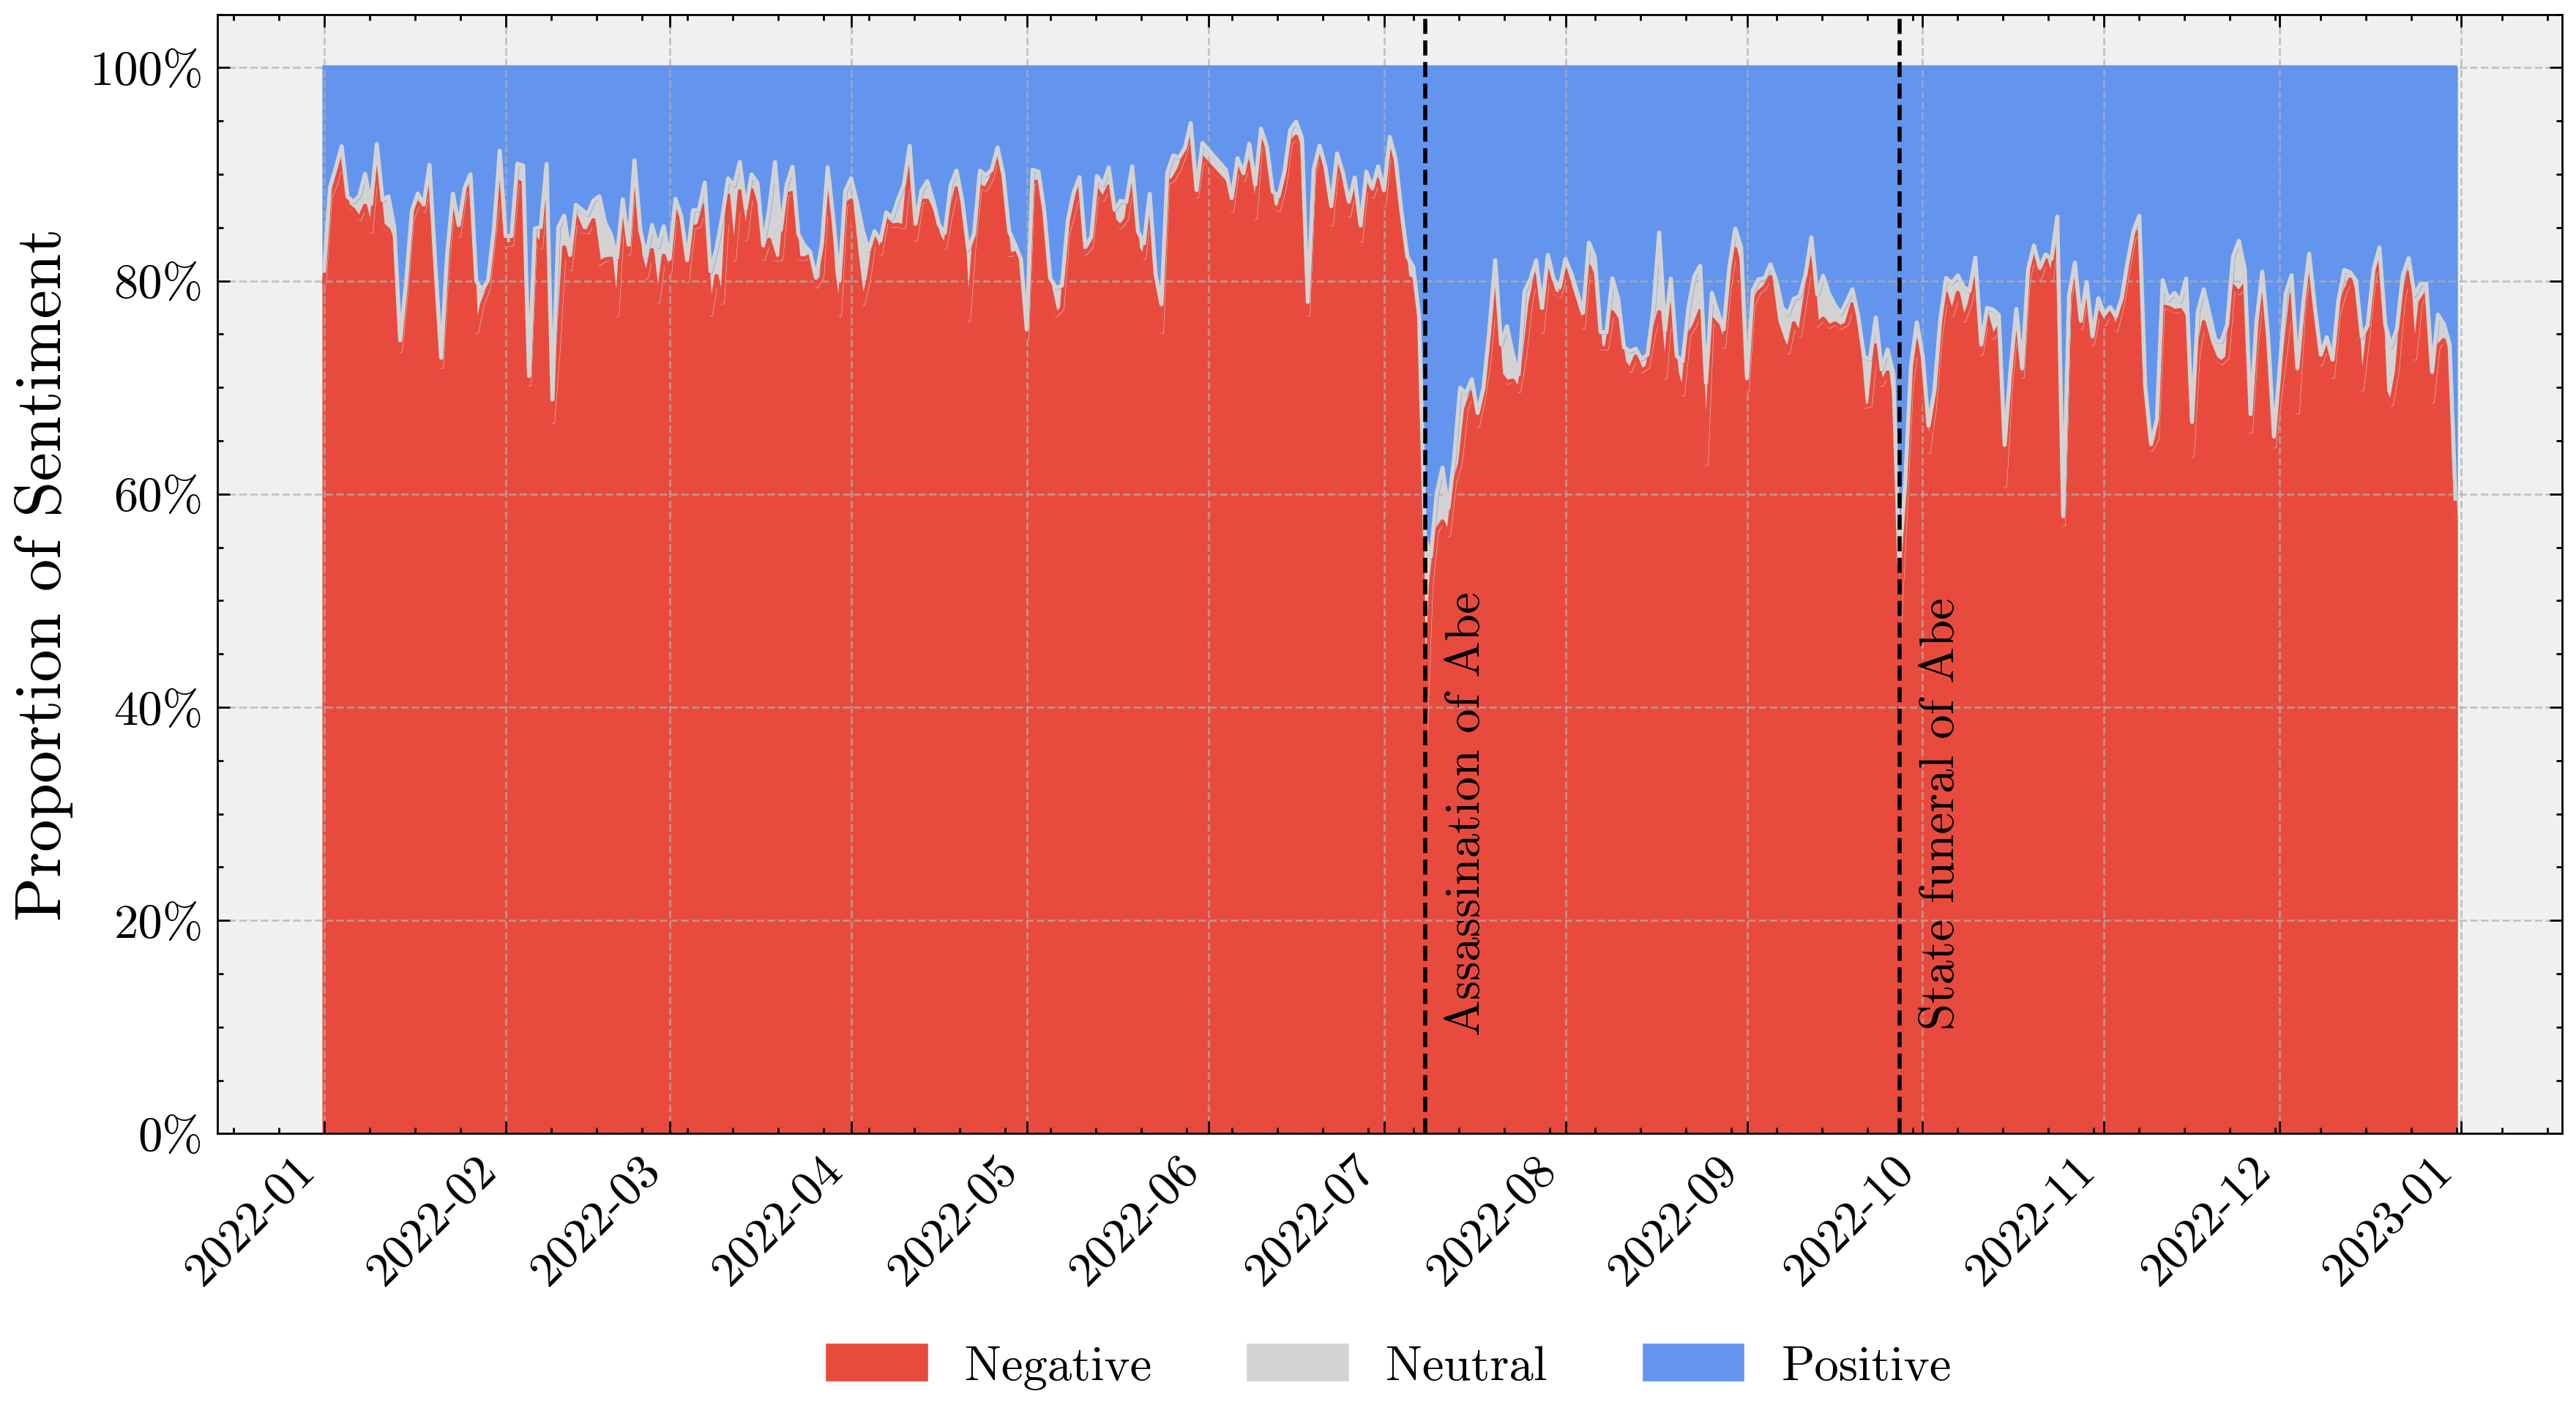
\includegraphics[width=\linewidth]{Figure/sentiment_over_time.png}
            \caption{ソーシャルメディアにおける長期的な意見変化}
            \label{fig:enter-label}
            \end{figure}
            \end{column}
        \end{columns}
    \end{frame}


    \begin{frame}{現在取り組んでいる研究}{モビリティデータによる社会的空間隔離の分析}
        \begin{columns}
        \begin{column}{0.5\textwidth}
                \begin{itemize}
                    \item \textbf{モビリティデータ}：モバイルセンサによる取得される位置情報
                    \pause
                    \item \textbf{社会的空間隔離}: 異なる社会集団が地理的に分離される
                    \begin{itemize}
                          \item 社会的分断
                          \item 機会の不平等
                     \end{itemize}

                \end{itemize}
        \end{column}        
        \begin{column}{0.5\textwidth}
            \begin{figure}
            \centering
            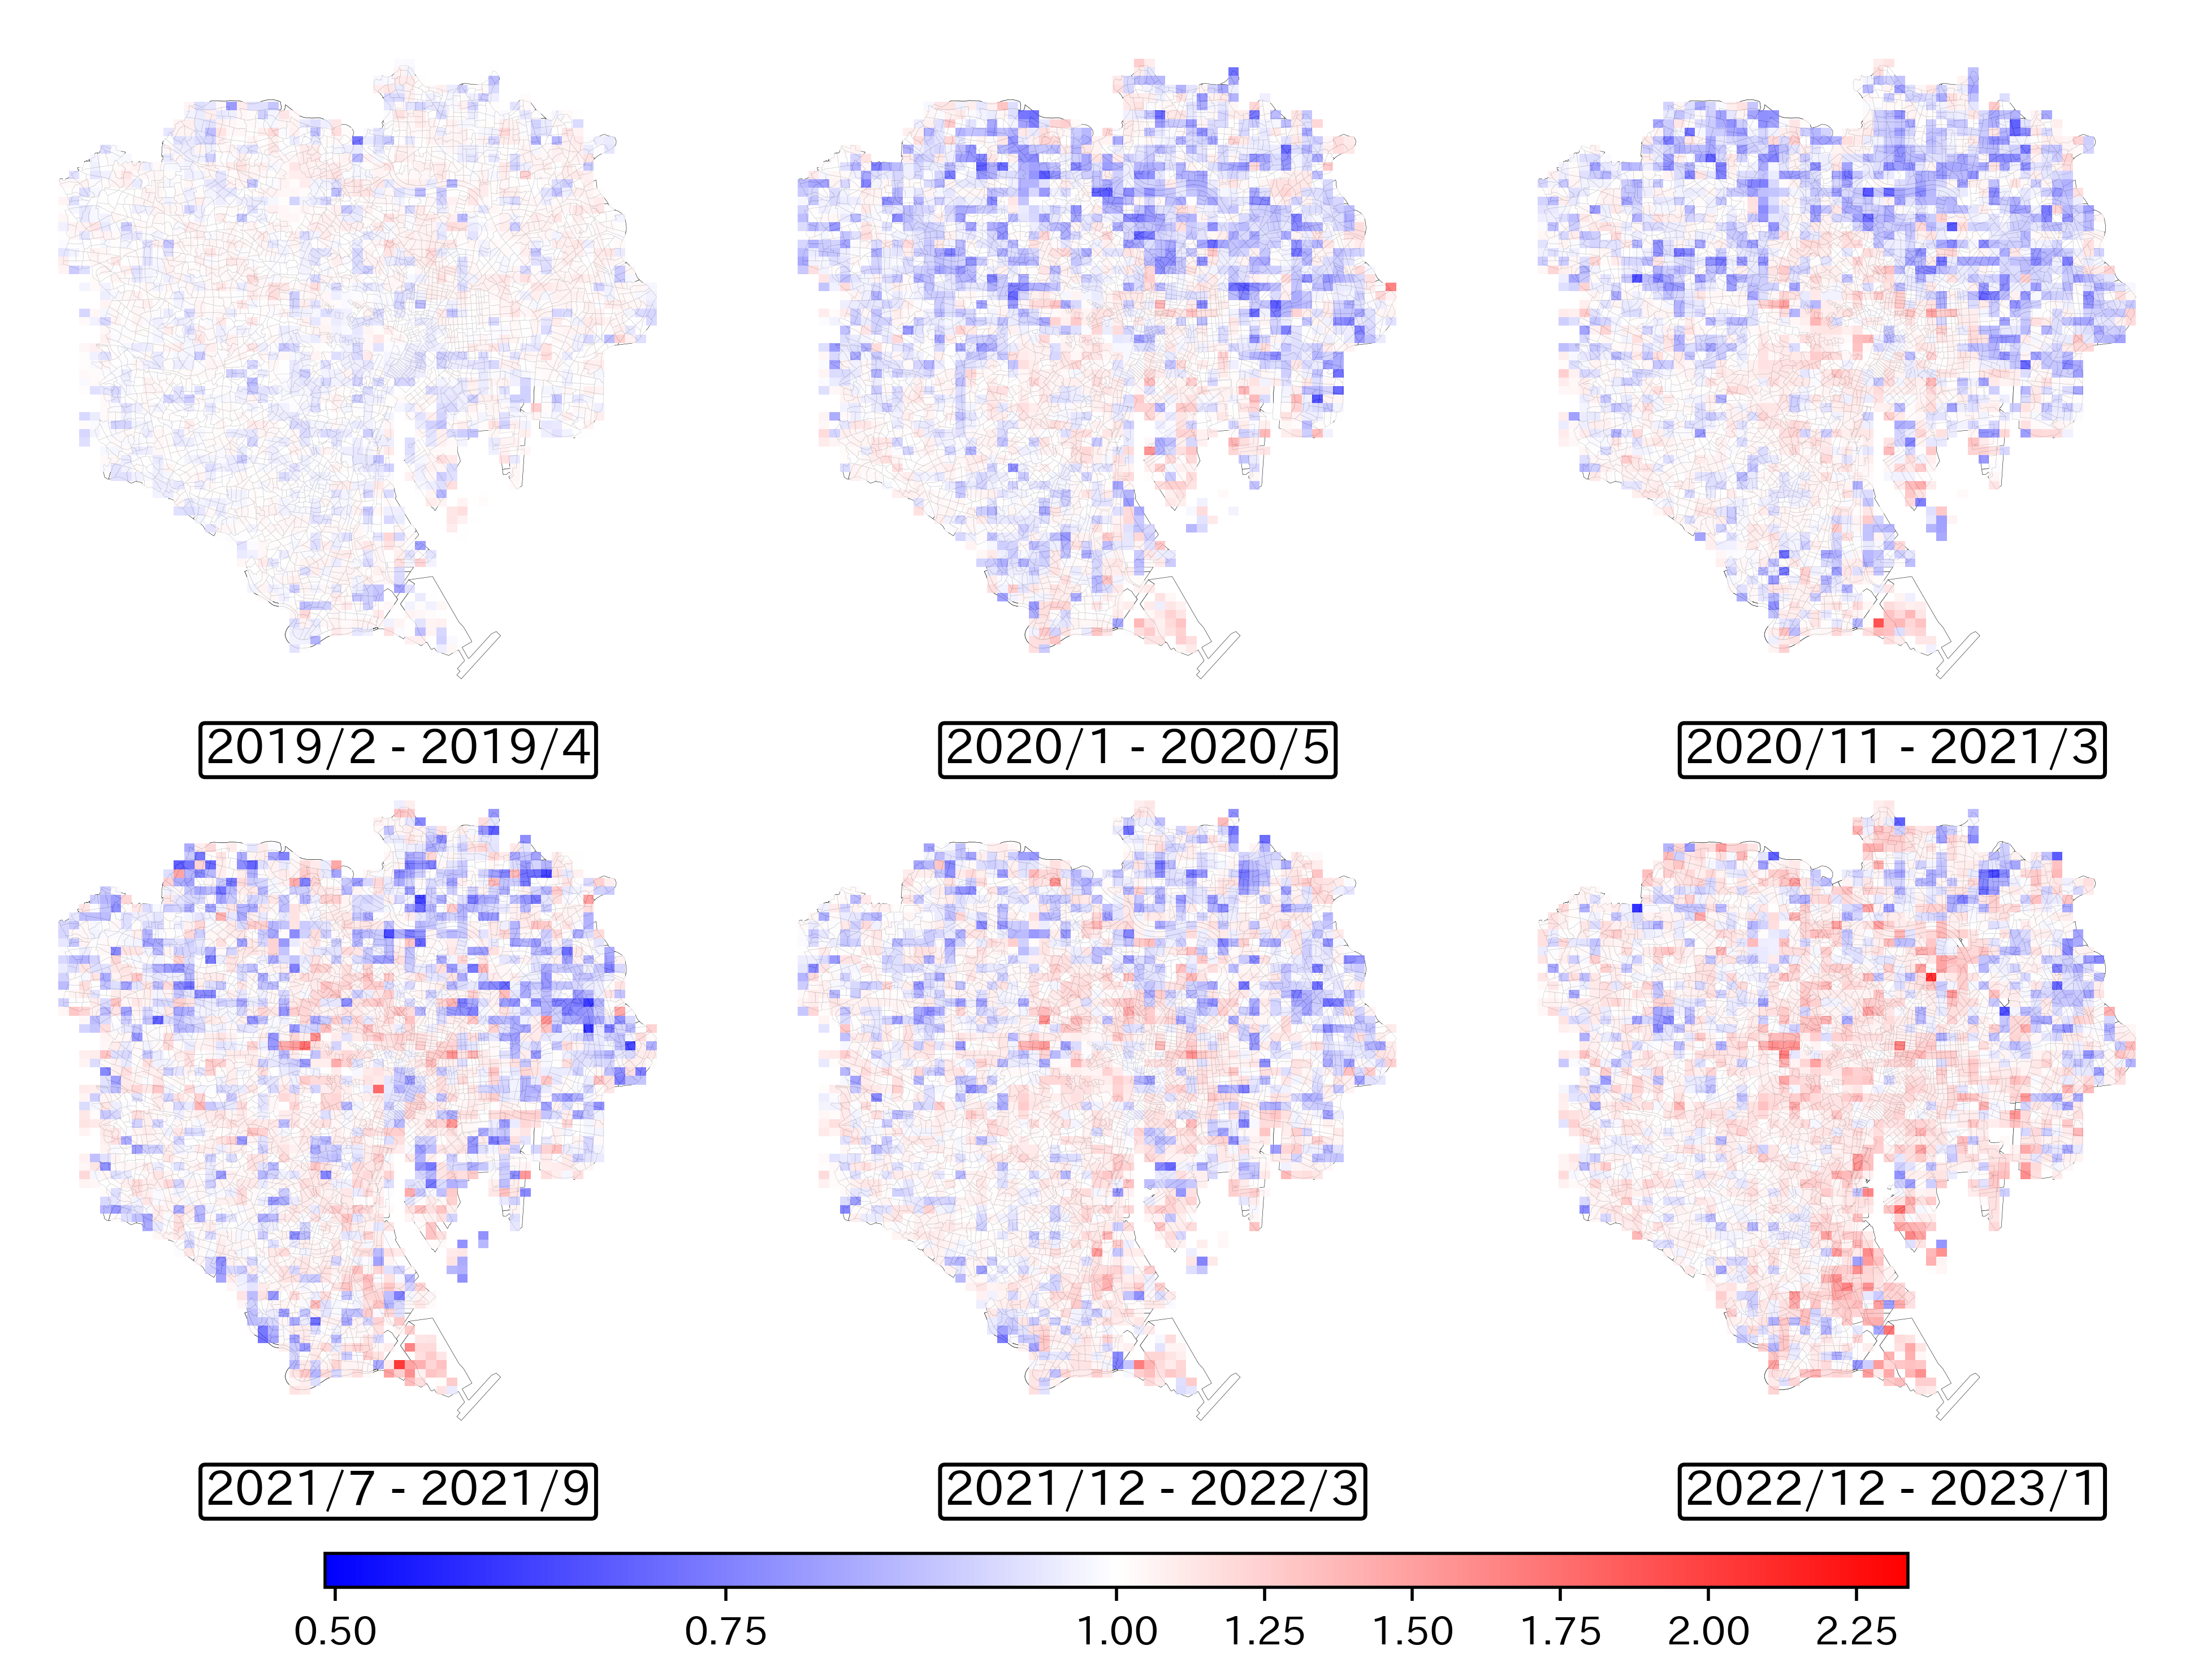
\includegraphics[width=\linewidth]{Figure/se_map.png}
            \caption{コロナにおける社会的空間隔離の推移}
            \label{fig:enter-label}
            \end{figure}
            \end{column}
        \end{columns}
    \end{frame}

\begin{frame}{現在取り組んでいる研究}{歴史資料に対するテキストマイニング}
    \begin{columns}
        \begin{column}{0.5\textwidth}
            \vspace{-0.5cm} % 调整文字和图像之间的间距
            \begin{minipage}[t][0.8\textheight][t]{\textwidth} % 设置统一高度
                \begin{itemize}
                    \item 歴史記録から天文・気象状況の特定と分析
                \end{itemize}
                \begin{figure}
                    \centering
                    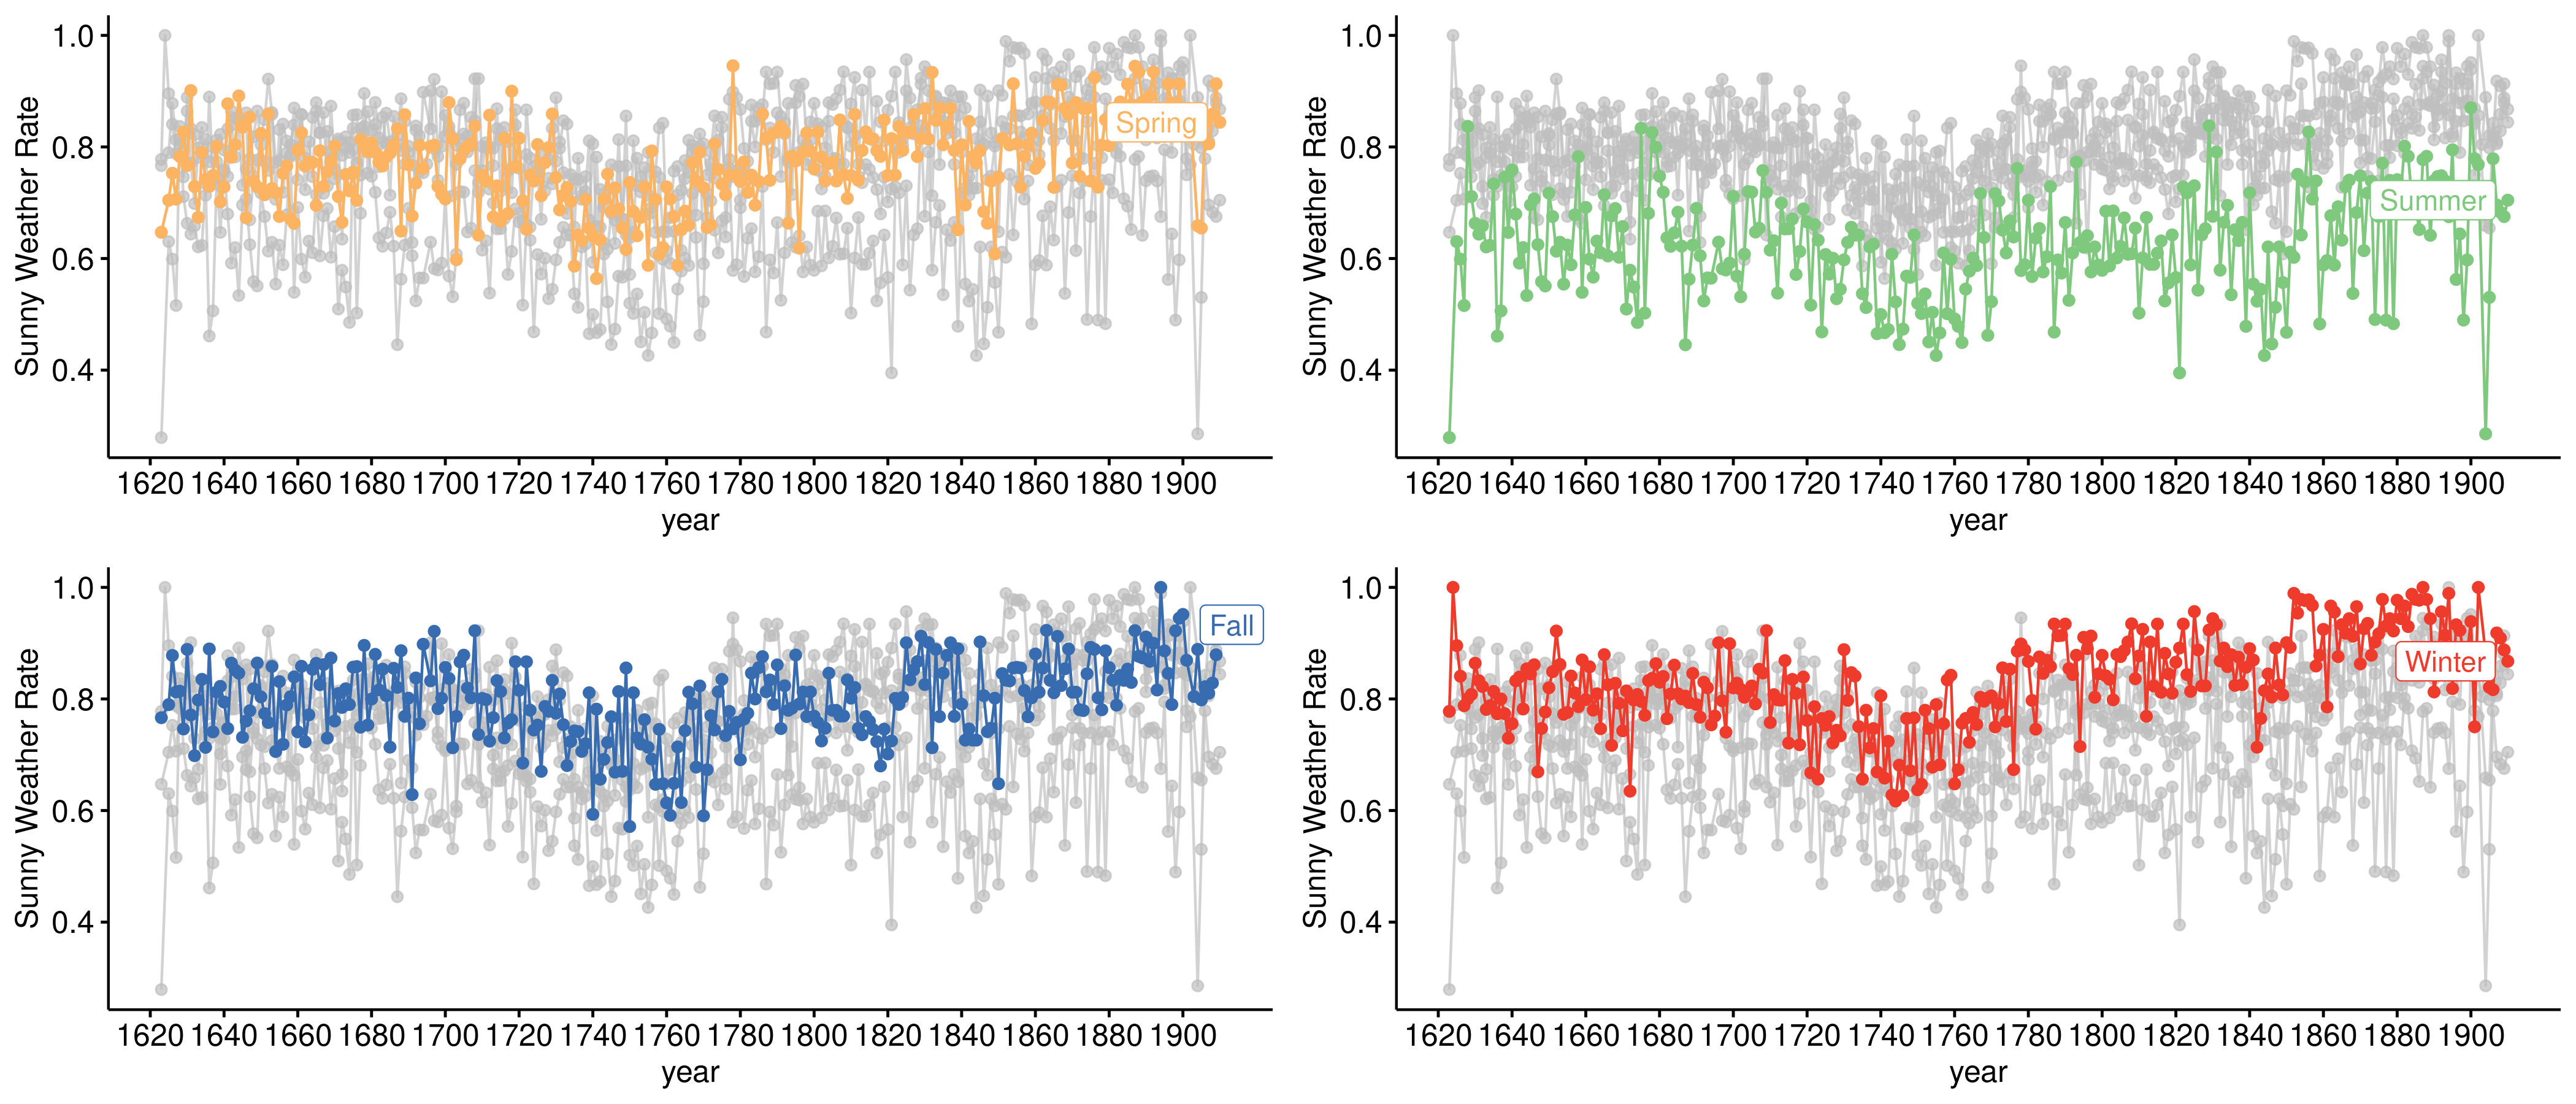
\includegraphics[width=0.9\linewidth]{Figure/p_rate.png}
                    \caption{歴史記録による特定した数百年間晴天率の推移}
                    \label{fig:enter-label}
                \end{figure}
            \end{minipage}
        \pause
        \end{column}
        \begin{column}{0.5\textwidth}
            \vspace{-0.5cm} % 调整文字和图像之间的间距
            \begin{minipage}[t][0.8\textheight][t]{\textwidth} % 设置统一高度
                \begin{itemize}
                    \item テキストによる集合表象・集合意識に対して定量的な測定
                \end{itemize}
                \begin{figure}
                    \centering
                    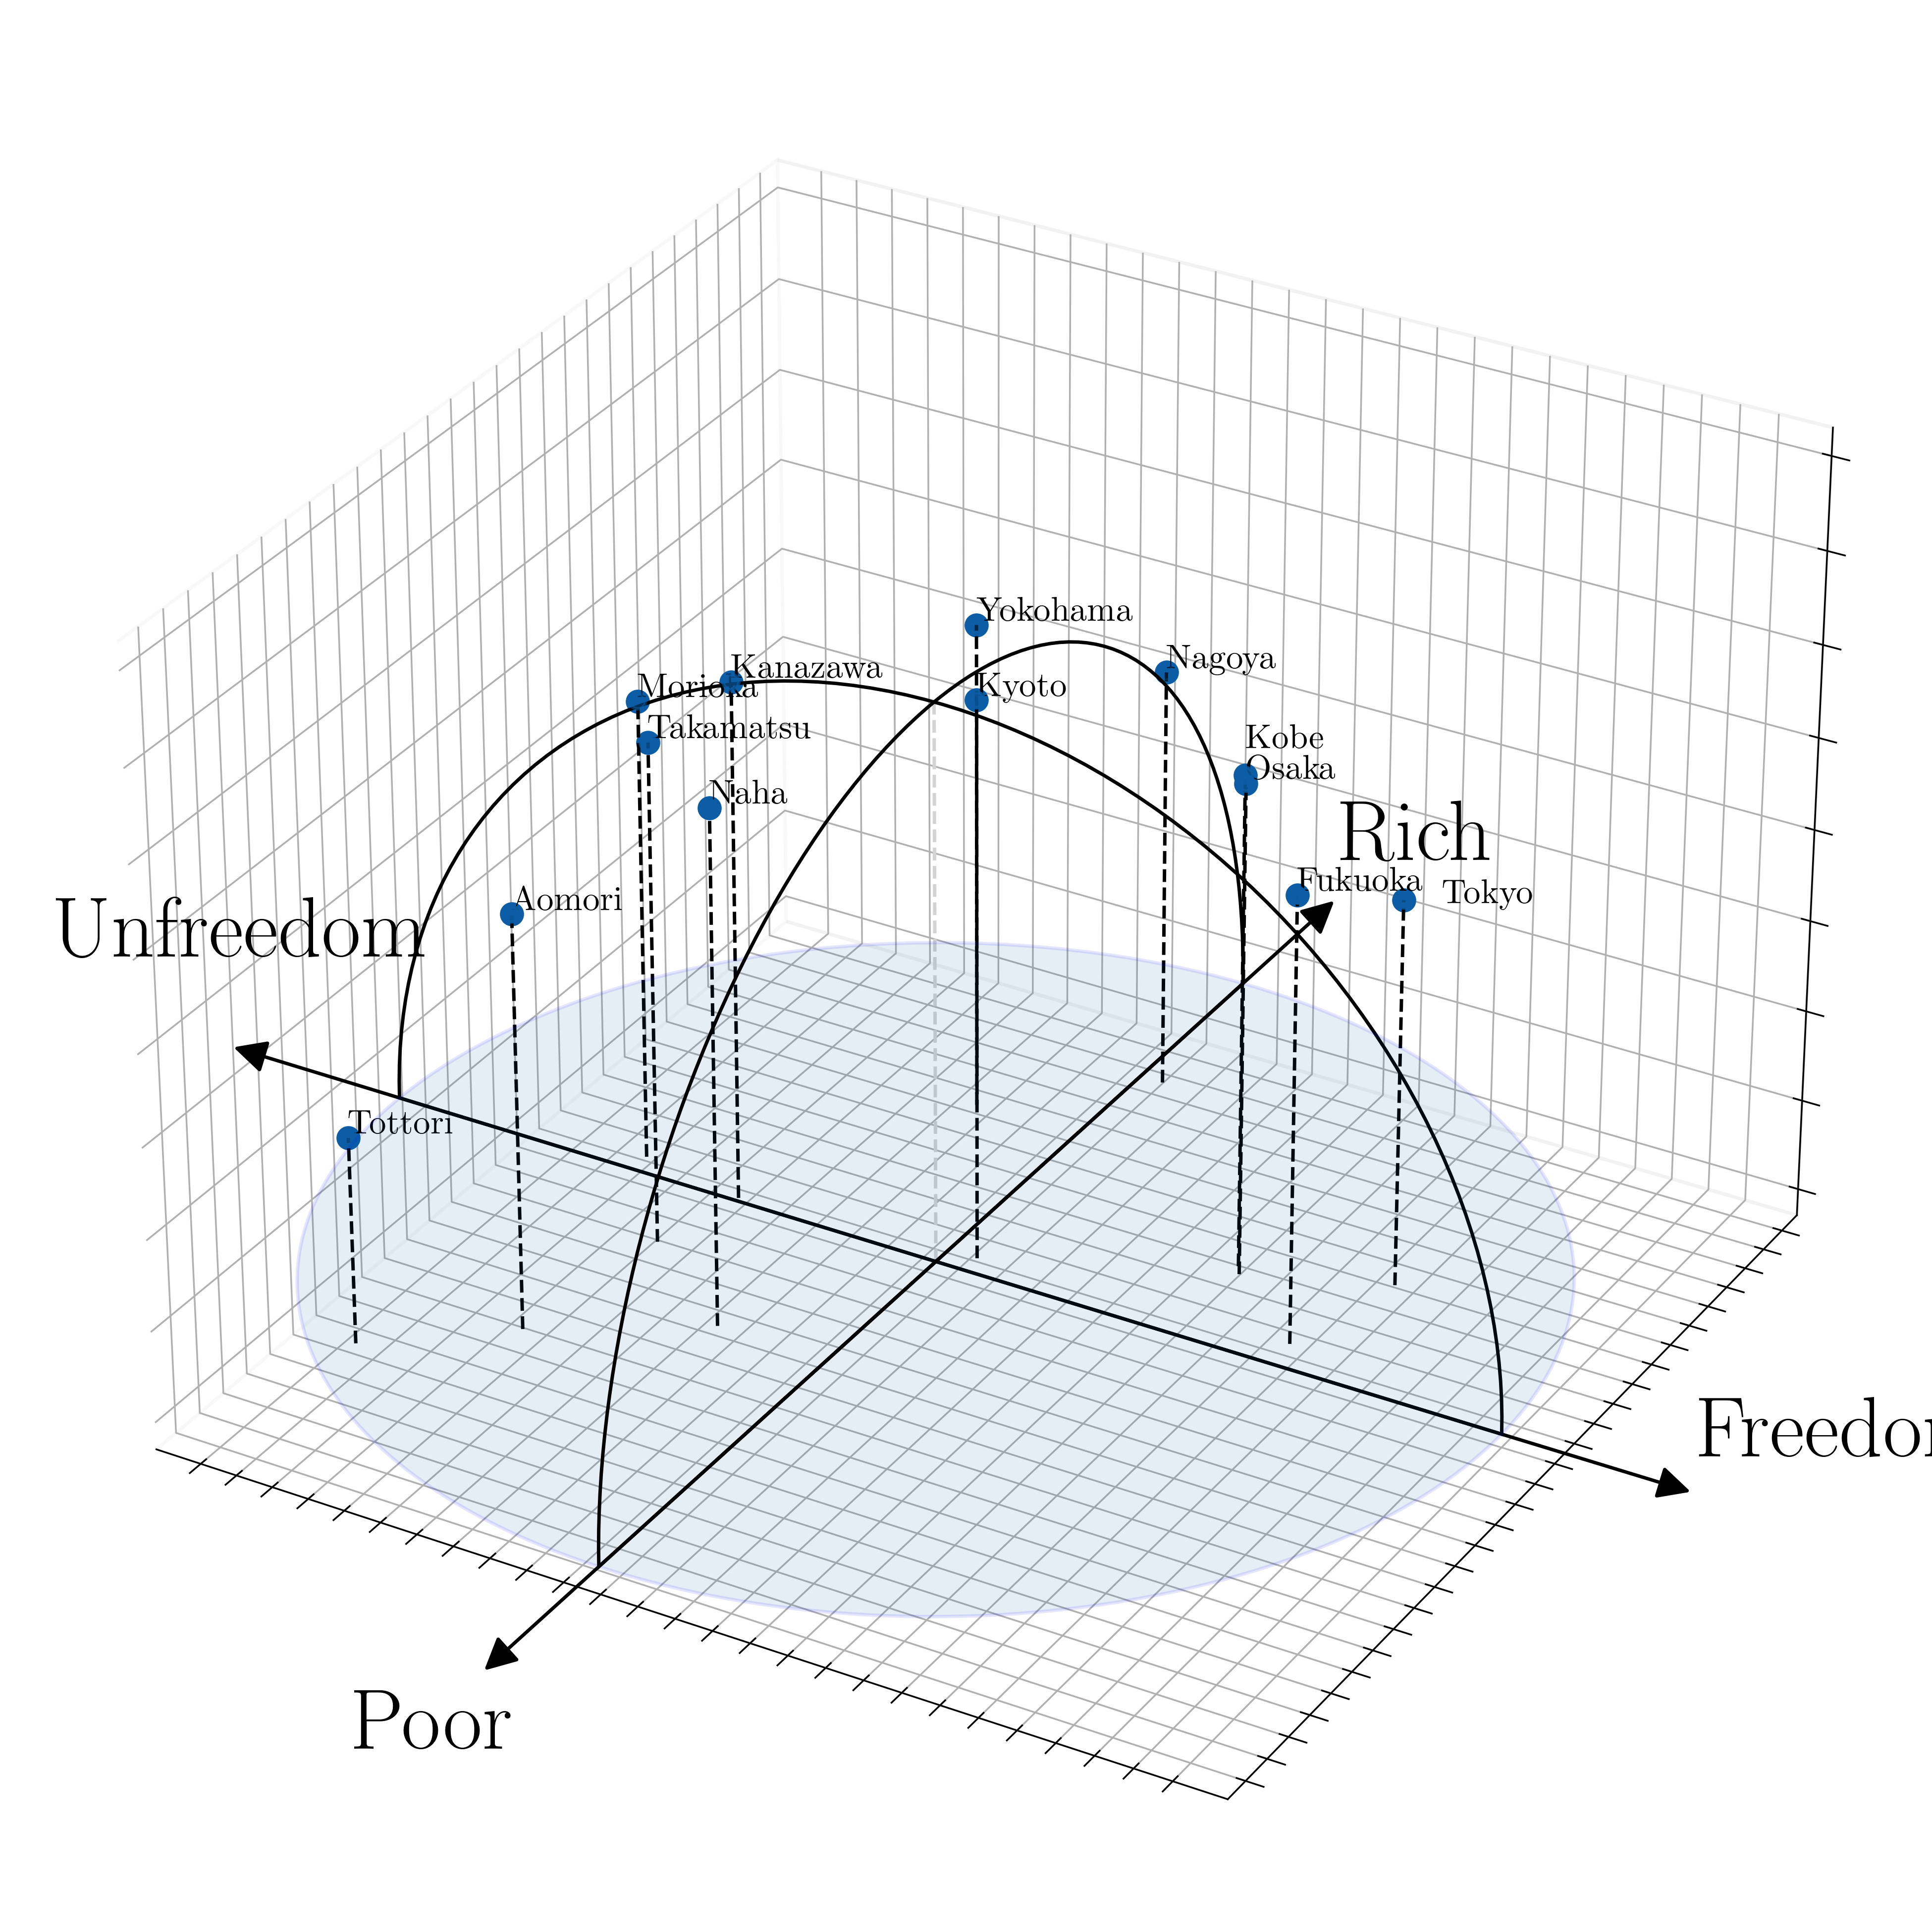
\includegraphics[width=0.55\linewidth]{Figure/rich_poor.png}
                    \caption{単語埋め込みによる意味空間の構築}
                    \label{fig:enter-label}
                \end{figure}
            \end{minipage}
        \end{column}
    \end{columns}
\end{frame}


    \section{計算社会科学の紹介}
    \begin{frame}{計算社会科学とは}{\secname}
    \begin{itemize}
        \item 計算社会科学とは、a)\textbf{デジタルな観察データ}（オンライン上の行動、IoT等により取得された物理的世界での行動、デジタル化された歴史資料や行政記録を含む）、b)\textbf{オンライン上の実験・サーベイデータ}、c)\textbf{数理・コンピュータモデリングに}よる分析、などを用いて、\textbf{社会現象のリアリティとメカニズムの解明}を試みる社会科学とコンピュータサイエンスの融合領域である(瀧川, 2018)
    \end{itemize}
    \rfootnote{瀧川 裕貴. (2018). 社会学との関係から見た計算社会科学の現状と課題. 理論と方法, 33(1), 132–148.}
    
    \end{frame}

    \begin{frame}{計算社会科学の(外在的)背景}{\secname}
    \begin{itemize}
        \item \textbf{社会のデータ化}
        \begin{itemize}
            \item 人々の行動や社会現象を詳細に記録した膨大なデータが蓄積された
        \end{itemize}
        \pause
        \item \textbf{情報技術とインフラの進展}
        \begin{itemize}
            \item 高性能コンピュータの進化
            \item 深層学習(人工知能)の発展
        \end{itemize}
    \end{itemize}
    
    \end{frame}

    \begin{frame}{計算社会科学の(内在的)背景}{\secname}
    \boldcolor{社会科学自身の問題点を克服するため方法論の革新への要請} (瀧川, 2023)
    \begin{itemize}
        \item \textbf{理論と実証の乖離}
        \begin{itemize}
            \item 実証研究で用いられるデータや方法と社会科学理論の方向性との齟齬の存在
            \item 行為者の複雑な相互作用や非線形効果の無視
        \end{itemize}
        \pause
        \item \textbf{分析手法の信頼性への疑問}
        \begin{itemize}
            \item 社会科学における因果推論の問題
            \item 再現可能性および一般化可能性の危機
        \end{itemize}

    \end{itemize}
    \rfootnote{瀧川 裕貴. (2023). 社会学方法論としての計算社会科学. 北田暁大, 岸政彦, 筒井淳也, 丸山里美, \& 山根純佳(編)  「理論・方法 岩波講座 社会学 第1巻」. 岩波書店.}
    \end{frame}

    \begin{frame}{計算社会科学の可能性}{\secname}
    \boldcolor{新しい社会学方法論としての計算社会科学の可能性} (瀧川, 2023)
    \begin{itemize}
        \item \textbf{データの可能性}
        \pause
        \item \textbf{因果メカニズムの解明可能性}
        \begin{itemize}
            \item 観察データによる因果推論
            \item デジタルフィールド実験
        \end{itemize}
        \pause
        \item \textbf{深層学習の科学方法論としての可能性}
        \begin{itemize}
            \item 仮説演繹モデルからの解放
            \item データの探索的分析
        \end{itemize}
        \pause
        \item \textbf{認知モデルの理論的可能性}
        \begin{itemize}
            \item 因果メカニズムの解明とはマクロ現象の背後に潜むマイクロなプロセスの特定のことであり、より具体的には人々が他者の行動や出来事の意味を解釈し（認知し）、判断を下し、そして行為するプロセスをモデルに組み込むこと
        \end{itemize}
    \end{itemize}
    \rfootnote{瀧川 裕貴. (2023). 社会学方法論としての計算社会科学. 北田暁大, 岸政彦, 筒井淳也, 丸山里美, \& 山根純佳(編)  「理論・方法 岩波講座 社会学 第1巻」. 岩波書店.}
    \end{frame}
    
    \section{大規模言語モデルの紹介}

    \begin{frame}{大規模言語モデルとは}{\secname}
    \begin{itemize}
        \item 大規模言語モデルとは、大量のテキストデータを学習して、自然言語を理解・生成する能力を持つ人工知能を指す
        \pause
        \begin{itemize}
            \item 与えられたトークン列(テキスト)に対して、次のトークン(テキスト)の生成される確率を予測するモデルである 「\boldcolor{G}enerative Model」
            \pause
            \item 大規模なテキストコーパスを使用して、言語モデルは言語に関する幅広い知識を獲得する 「\boldcolor{P}re-trained」
            \pause
            \item \boldcolor{T}ransformerアーキテクチャ：文脈情報をを効率的に捉えつつ、並列計算で高速な処理が可能
        \end{itemize}
    \end{itemize}
    \end{frame}

    \begin{frame}{大規模言語モデルの社会科学における応用可能性}{\secname}
    \begin{itemize}
        \item 社会学の目標は\textbf{マクロ現象の因果メカニズム}の実証的解明
        \begin{itemize}
            \item メカニズムを明らかにするとは，人々の相互行為や関係性，つながりの形成といったマイクロなプロセスに言及して説明すること
        \end{itemize}
        \pause
        \item \textbf{大規模言語モデルがもたらす可能性}
        \begin{itemize}
            \item \boldcolor{テキストマイニング}: デジタル観察データによる社会現象の生成メカニズムを因果的に明らかにすること
            \pause
            \item \boldcolor{実験}: 人工知能や計算言語学の認知モデルを参照しつつ、行為者が他者の行為や社会的出来事の意味を解釈し，それに基づいて自らの行為を選択するプロセスをモデル化すること
            \pause
            \item \boldcolor{社会シミュレーション}：演繹モデルから脱却することでデータからの発見に基づくグラウンディッドな理論構築を行うこと
        \end{itemize}
    \end{itemize}
    \end{frame}

    \section{大規模言語モデルの応用}

    \begin{frame}{テキストマイニングと社会科学}{\secname : テキストマイニング}
    \begin{itemize}
        \item テキストマイニングは文書データから有用な情報を発見する方法として社会科学的な分析にも広く用いられている
        \end{itemize}
        \begin{columns}[c]
        \begin{column}{0.5\textwidth}
        \begin{minipage}[t][0.8\textheight][t]{\textwidth} % 设置统一高度
        \centering
        \vspace{0.5cm} % 可根据需求调整高度
        \textbf{感情分析}
        \begin{figure}
            \centering
            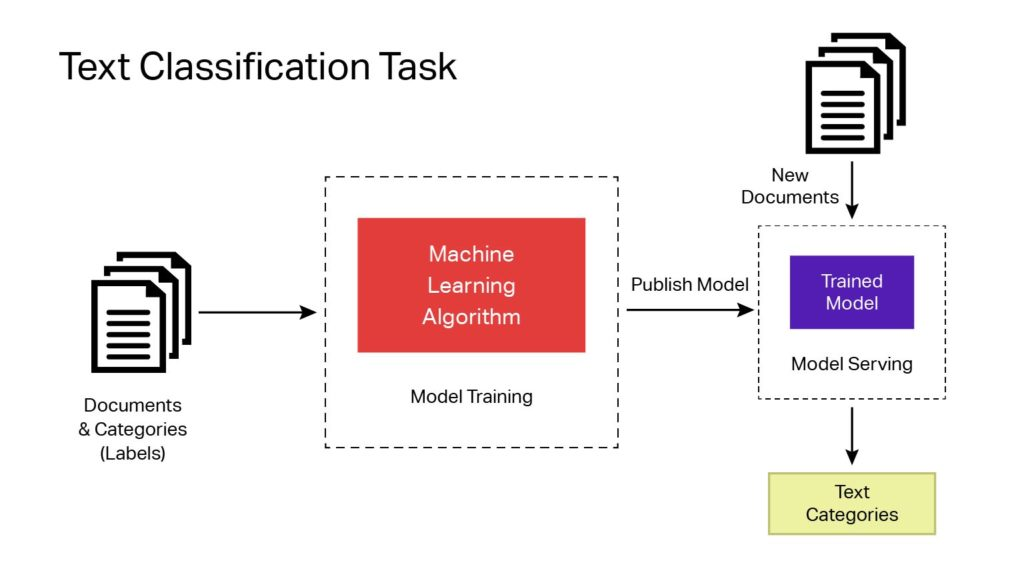
\includegraphics[width=0.8\linewidth]{Figure/Text-Classification-Dataset-Repositories-1024x567.jpg}
        \end{figure}
        \end{minipage}
        \end{column}
    
        \begin{column}{0.5\textwidth}
        \begin{minipage}[t][0.8\textheight][t]{\textwidth} % 设置统一高度
        \centering
        \vspace{0.5cm} % 可根据需求调整高度
        \textbf{トピックモデル}
        \begin{figure}
            \centering
            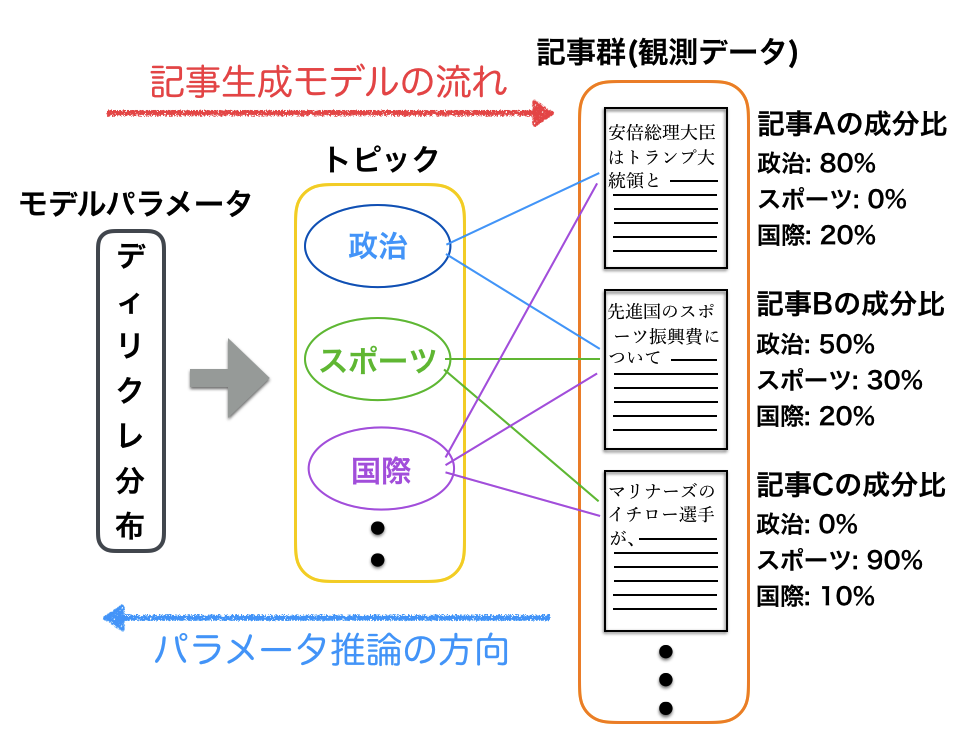
\includegraphics[width=0.8\linewidth]{Figure/topic_model.png}
        \end{figure}
        \end{minipage}
        \end{column}
        \end{columns}
    \end{frame}

    \begin{frame}{既存手法の問題点}{\secname : テキストマイニング}
    \begin{itemize}
        \item \textbf{テキスト分析の精度}
        \begin{itemize}
            \item 長文や複雑な文章の解析が難しい:文脈、文法構造、多義語の扱いが不十分
        \end{itemize}
        \pause
        \vspace{0.5cm}
        \item \textbf{非効率性}: 学習済みモデルを特定のタスクの適用するためにはファインチューニングなどの追加学習が必要
        \begin{itemize}
            \item ドメイン依存性が高い
            \item 多言語対応のコストが高い
            \item (大量の)教師データの作成が必要
        \end{itemize}
    \end{itemize}
    \end{frame}
        
    \begin{frame}{大規模言語モデルによるテキストマイニングの革新}{\secname : テキストマイニング}
        \begin{columns}
        \begin{column}{0.5\textwidth}
                \begin{itemize}
                    \item \boldcolor{In-context learning}：\textbf{与えられた入力のコンテキストに基づいて新しいタスクを理解し、適応する能力}
                    \pause
                    \begin{itemize}
                          \item Zero-shotやFew-shot学習により、少量のデータでも高い性能を発揮
                          \item 特定のドメインや言語に対応する際には、ファインチューニングを行うだけで十分な精度を達成できる
                     \end{itemize}

                \end{itemize}
        \end{column}        
        \begin{column}{0.5\textwidth}
            \begin{figure}
            \centering
            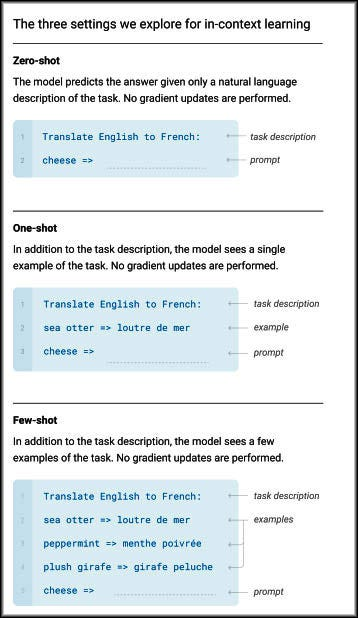
\includegraphics[width=0.5\linewidth]{Figure/in-context.png}
            \end{figure}
            \end{column}
        \end{columns}
    \end{frame}
    
    \begin{frame}{大規模言語モデルによるテキストマイニングの革新}{\secname : テキストマイニング}
        \begin{figure}
            \centering
            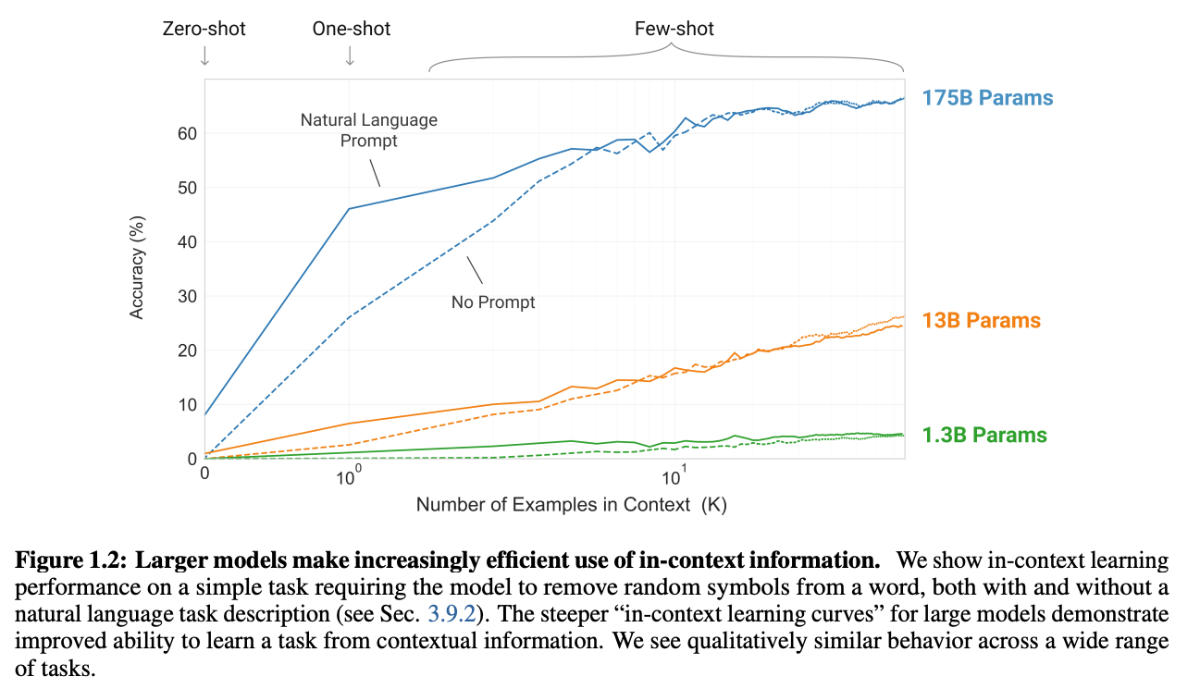
\includegraphics[width=0.8\linewidth]{Figure/gpt-accuracy.png}
            \label{fig:enter-label}
        \end{figure}
        \rfootnote{Brown, T. B., Mann, B., Ryder, N., et al. (2020). Language Models are Few-Shot Learners. ArXiv. \href{https://arxiv.org/abs/2005.14165}{https://arxiv.org/abs/2005.14165}}
    \end{frame}

    \begin{frame}{Best Practice: プロンプトエンジニアリング}{\secname : テキストマイニング}
        \begin{figure}
            \centering
            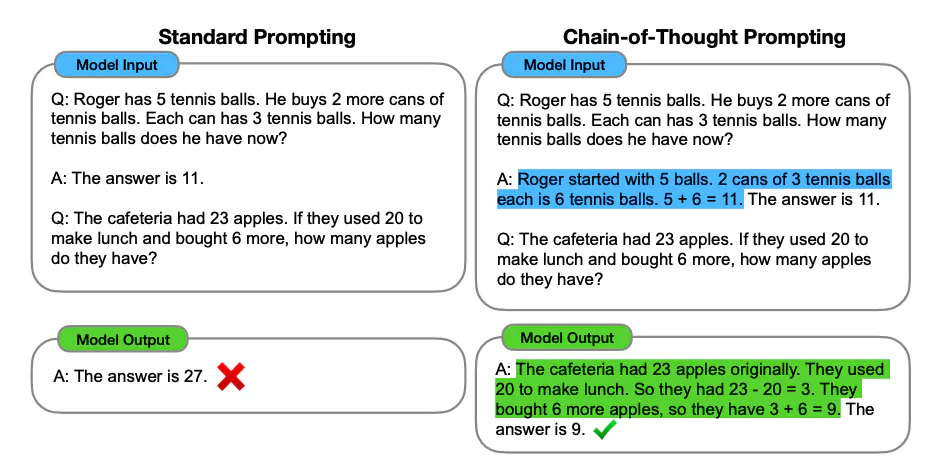
\includegraphics[width=0.8\linewidth]{Figure/cot.png}
            \label{fig:enter-label}
        \end{figure}
        \rfootnote{Wei, J., Wang, X., Schuurmans, D., et al. (2022). Chain-of-Thought Prompting Elicits Reasoning in Large Language Models. ArXiv. \href{https://arxiv.org/abs/2201.11903}{https://arxiv.org/abs/2201.11903}}
    \end{frame}

    \begin{frame}{Best Practice: プロンプトエンジニアリング}{\secname : テキストマイニング}
        \begin{figure}
            \centering
            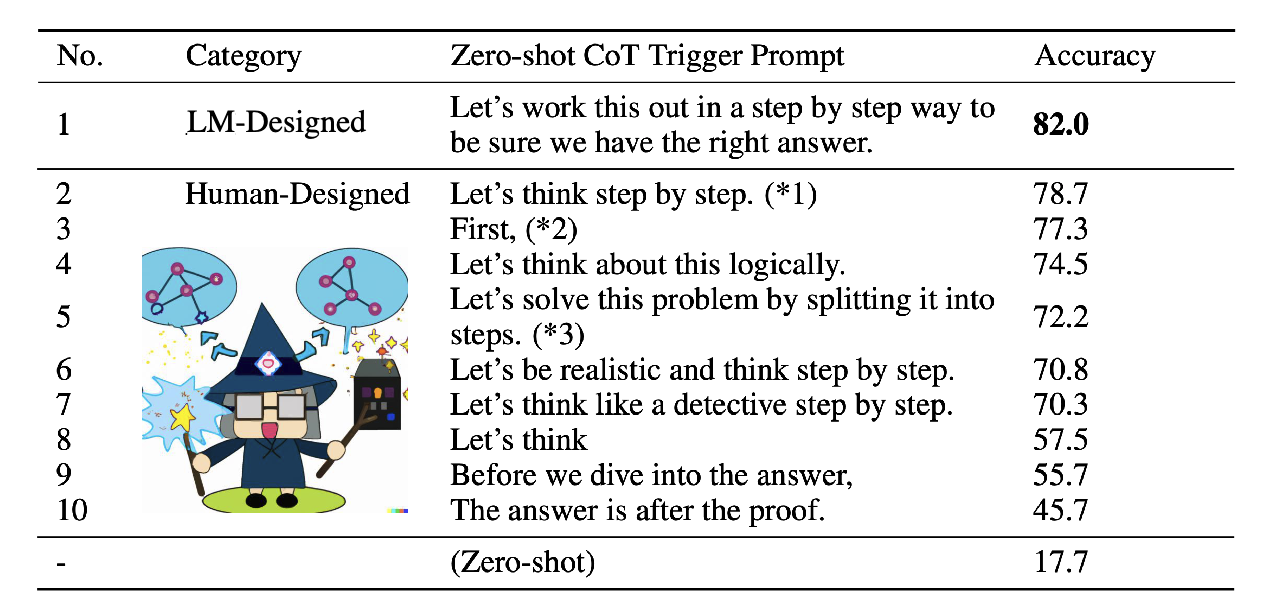
\includegraphics[width=0.8\linewidth]{Figure/cot_prompting.png}
            \label{fig:enter-label}
        \end{figure}
        \rfootnote{source: \href{https://research.google/blog/language-models-perform-reasoning-via-chain-of-thought/}{Language Models Perform Reasoning via Chain of Thought}}
    \end{frame}

    \begin{frame}{Best Practice:量子化LLMに対するファインチューニング}{\secname : テキストマイニング}
    \begin{itemize}
        \item 大規模言語モデルの学習と推論は非常に\textbf{大量の計算リソースとメモリを必要とする}
        \pause
        \begin{itemize}
            \item 個人用なPCやサーバではほぼ無理
            \item 有料なAPIを使う選択肢もあるが
        \end{itemize}
        \pause
        \item 大規模言語モデル（LLM）の効率性を向上させるために、モデルのパラメータを低精度で表現する技術（量子化）を行った後、\textbf{特定のタスクに最適化するためにファインチューニング}
        \pause
        \begin{itemize}
            \item 量子化を行った後、モデルの性能が多少低下することがあるが、リソースが限られたデバイスでも大規模な言語モデルを実行できるようになる
            \item 効率的的にファインチューニング手法：LoRA（Low-Rank Adaptation）
        \end{itemize}
    \end{itemize}
    \end{frame}

    \begin{frame}{Best Practice:量子化LLMに対するファインチューニング}{\secname : テキストマイニング}
    \begin{itemize}
        \item テキスト分類（センチメント分析）
        \begin{itemize}
            \item 437 万9,962 のツイートから 1 万3,000 のツイート をランダムサンプリングにより取り出す。
            \item ネガティブ，ニュートラル，ポジティブのセンチメントラベル(「正解」ラベル)を一部付与 
            \item センチメント付与のルールブックを作成
            \item 正解ラベル付きデータセットの作成
        \end{itemize}
    \end{itemize}
    \rfootnote{瀧川裕貴, 永吉希久子, 呂沢宇, 下窪拓也, 渡辺誓司, 中村美子 ( 2023). ソーシャルメディア言論分析の方法①：2020年1月から辞任までの安倍首相に対するTwitter上の投稿分析を事例として,『放送研究と調査』3月号, 70-85
}
    \end{frame}

    \begin{frame}{Best Practice:量子化LLMに対するファインチューニング}{\secname : テキストマイニング}
\begin{table}
%\caption{Performance of stance detection with different models}
\centering
\resizebox{\textwidth}{!}{%
\begin{tabular}{lllll}
\hline
\textbf{Model}                       & \textbf{Positive} & \textbf{Neutral} & \textbf{Negative} & \textbf{All}     \\ \hline
tohoku-nlp/bert-large-japanese-v2                           & 58.12\%  & 48.13\% & 90.95\%  & 84.50\% \\
rinna/japanese-roberta-base                                 & 70.67\%  & 51.56\% & 92.57\%  & 86.94\% \\
stabilityai/japanese-stablelm-base-alpha-7b (Zero-shot)     & 29.00\%  & 1.5\%   & 42.69\%  & 35.46\% \\
\textbf{stabilityai/japanese-stablelm-base-alpha-7b (QLoRA)}         & 79.00\%  & 61.74\% & 95.06\%  & 90.09\% \\
Qwen/Qwen2.5-14B-Instruct (Zero-shot)                       & 36.16\%  & 40.59\% & 90.37\%  & 81.29\% \\
\textbf{Qwen/Qwen2.5-14B-Instruct (QLoRA)}                          & 81.46\%  & 56.28\% & 95.72\%  & 91.72\%  \\
tokyotech-llm/Llama-3.1-Swallow-8B-Instruct-v0.1(Zero-shot) & 51.13\%  & 23.38\% & 91.36\%  & 83.72\% \\
\textbf{tokyotech-llm/Llama-3.1-Swallow-8B-Instruct-v0.1(QLoRA)}     & 82.02\%  & 60.66\% & 95.86\%  & 92.04\% \\ \hline
\end{tabular}%
}
\label{fine-tuning}
\end{table}
\end{frame}

    \begin{frame}{ビネット実験}{\secname : 実験}
    \begin{itemize}
        \item \textbf{ヴィネット実験}とは、特定の状況やシナリオを模倣した「ヴィネット」（短いストーリーや事例）を被験者に提示し、状況や事例に対する評価や認識を回答させる。
        \begin{itemize}
            \item ある人物の行動が倫理的に正当かどうかを評価させる
            \item 政策に対する市民の反応
        \end{itemize}
        \pause
        \item \textbf{ヴィネット実験に関する課題}
        \begin{itemize}
            \item シナリオ作成にかかる労力
            \item 現実との乖離
            \item 被験者の解釈のばらつき
        \end{itemize}
    \end{itemize}
    \end{frame}

    \begin{frame}{ビネット実験の略歴生成として利用}{\secname : 実験}
    \begin{block}{架空の人生略歴を読んで、人生の幸福度を評価してもらう}
    性別:男性，業種:テクノロジー，学歴:修士，きょうだいの数:4，婚姻状態:離別，子どもの数:3，出身階層の暮らし向き(5段階：上，中の上，中の中，中の下，下):中の上，寿命:46，ウェルビーイングの11の要素 富:5，健康:5，安全:5，友人関係:5，学びの喜び:5，自由:5，（主人公のいる社会の）民主主義:5，遊び:5，自然:5，（主人公のいる社会の）平和:5，快楽:5．        
    \end{block}
    \pause
    \begin{block}{生成した略歴}
    彼は中流上階層の家庭に5人きょうだいの長男として生まれました。幼少期から知的な好奇心が旺盛で、家族と過ごす時間や友人たちとの交流の中で、自然や科学に触れる機会が多くありました。...
    
    修士課程まで進学し、情報工学分野の研究に没頭しました。彼はさまざまなプロジェクトに参加し、国内外で活躍する研究仲間たちと切磋琢磨しながら、研究を深めていきました。
    \end{block}
    
    \end{frame}

    \begin{frame}{ビネット実験における大規模言語モデルの活用}{\secname : 実験}
    \begin{itemize}
        \item \textbf{多様なシナリオ生成}
        \begin{itemize}
            \item シナリオ作成の負担が大幅に軽減
            \item 回答者の個別の属性に基づいてヴィネットの内容を微調整
            \item 現実世界の文脈に基づくシナリオ生成
        \end{itemize}
        \pause
        \item \textbf{シナリオの解釈と標準化}
        \begin{itemize}
            \item シナリオの一貫性
            \item 大規模言語モデルの予測反応による実験デザインの改善
        \end{itemize}
    \end{itemize}
    \end{frame}

% Social Simulation

    \begin{frame}{Agent-based Models (ABMs)}{\secname : 社会シミュレーション}
    \begin{itemize}
        \item 社会シミュレーション: 計算モデルを活用して、社会的な現象やプロセスを再現・分析
        \begin{itemize}
            \item 個人や集団の相互作用や社会構造が、時間の経過とともにどのように進化するのかを理解
            \item  社会的政策や環境変化などの介入がどのような影響を及ぼすかを予測
        \end{itemize}
    \end{itemize}
    \pause
    \begin{itemize}
        \item ABMは、特定の環境内で個々のエージェントの相互作用をシミュレーションする計算モデル
        \begin{itemize}
        \item 各エージェントは定められたルールに従い、他のエージェントや環境との相互作用に基づいて自分の行動や特性を適応させることができる
        \item 個々のエージェントの行動や相互作用から、マクロ社会現象が自然に現れる
        \end{itemize}
    \end{itemize}
    \end{frame}

    \begin{frame}{ABMsによる意見形成の分析}{\secname : 社会シミュレーション}

    \begin{itemize}
        \item Hegselmann-Krauseモデルにおける意見更新ルール
        \begin{itemize}
            \item 距離のしきい値$\epsilon>0$を設定し、エージェント$i$は条件$|x_i - x_j| \leq \epsilon$を満たすエージェント$j$と相互作用する
            \item エージェント$i$の意見$x_i$は、相互作用範囲内にいる他のエージェントの意見の平均に更新される: $x_i(t+1) = \frac{1}{|N_i(t)|} \sum_{j \in N_i(t)} x_j(t)$
        \end{itemize}
        \pause
        \item Hegselmann-Krauseモデルの拡張
        \begin{itemize}
            \item 意見の影響力の導入 $x_i(t+1) = \frac{\sum_{j \in N_i(t)} w_{ij} x_j(t)}{\sum_{j \in N_i(t)} w_{ij}}$
            \item 動的な相互作用範囲 $\epsilon_i(t) = \epsilon_0 \cdot (1 + \alpha_i(t))$
            \item ノイズやランダム性の追加 $x_i(t+1) = \frac{1}{|N_i(t)|} \sum_{j \in N_i(t)} x_j(t) + \eta_i(t)$
        \end{itemize}
    \end{itemize}
 
    \end{frame}

    \begin{frame}{既存社会シミュレーション方法の問題点}{\secname : 社会シミュレーション}
    \begin{itemize}
        \item 従来のABMは抽象的な理論や単純化された仮定、事前定義されたルールに依存
        \begin{itemize}
            \item 現実世界の複雑な相互作用を十分に反映できず
            \item 異なる環境でのシミュレーションを支える汎用的なエージェントを設計することが困難であり、一般化が難しい
        \end{itemize}
    \end{itemize}

    \end{frame}

    \begin{frame}{大規模言語モデル駆動のエージェント}{\secname : 社会シミュレーション}
    \begin{itemize}
        \item 大規模のコーパスから得られた広範な知識や概念を基盤として、人間の行動と意思決定を再現するエージェントモデル
    \end{itemize}
    \begin{figure}
    \centering
    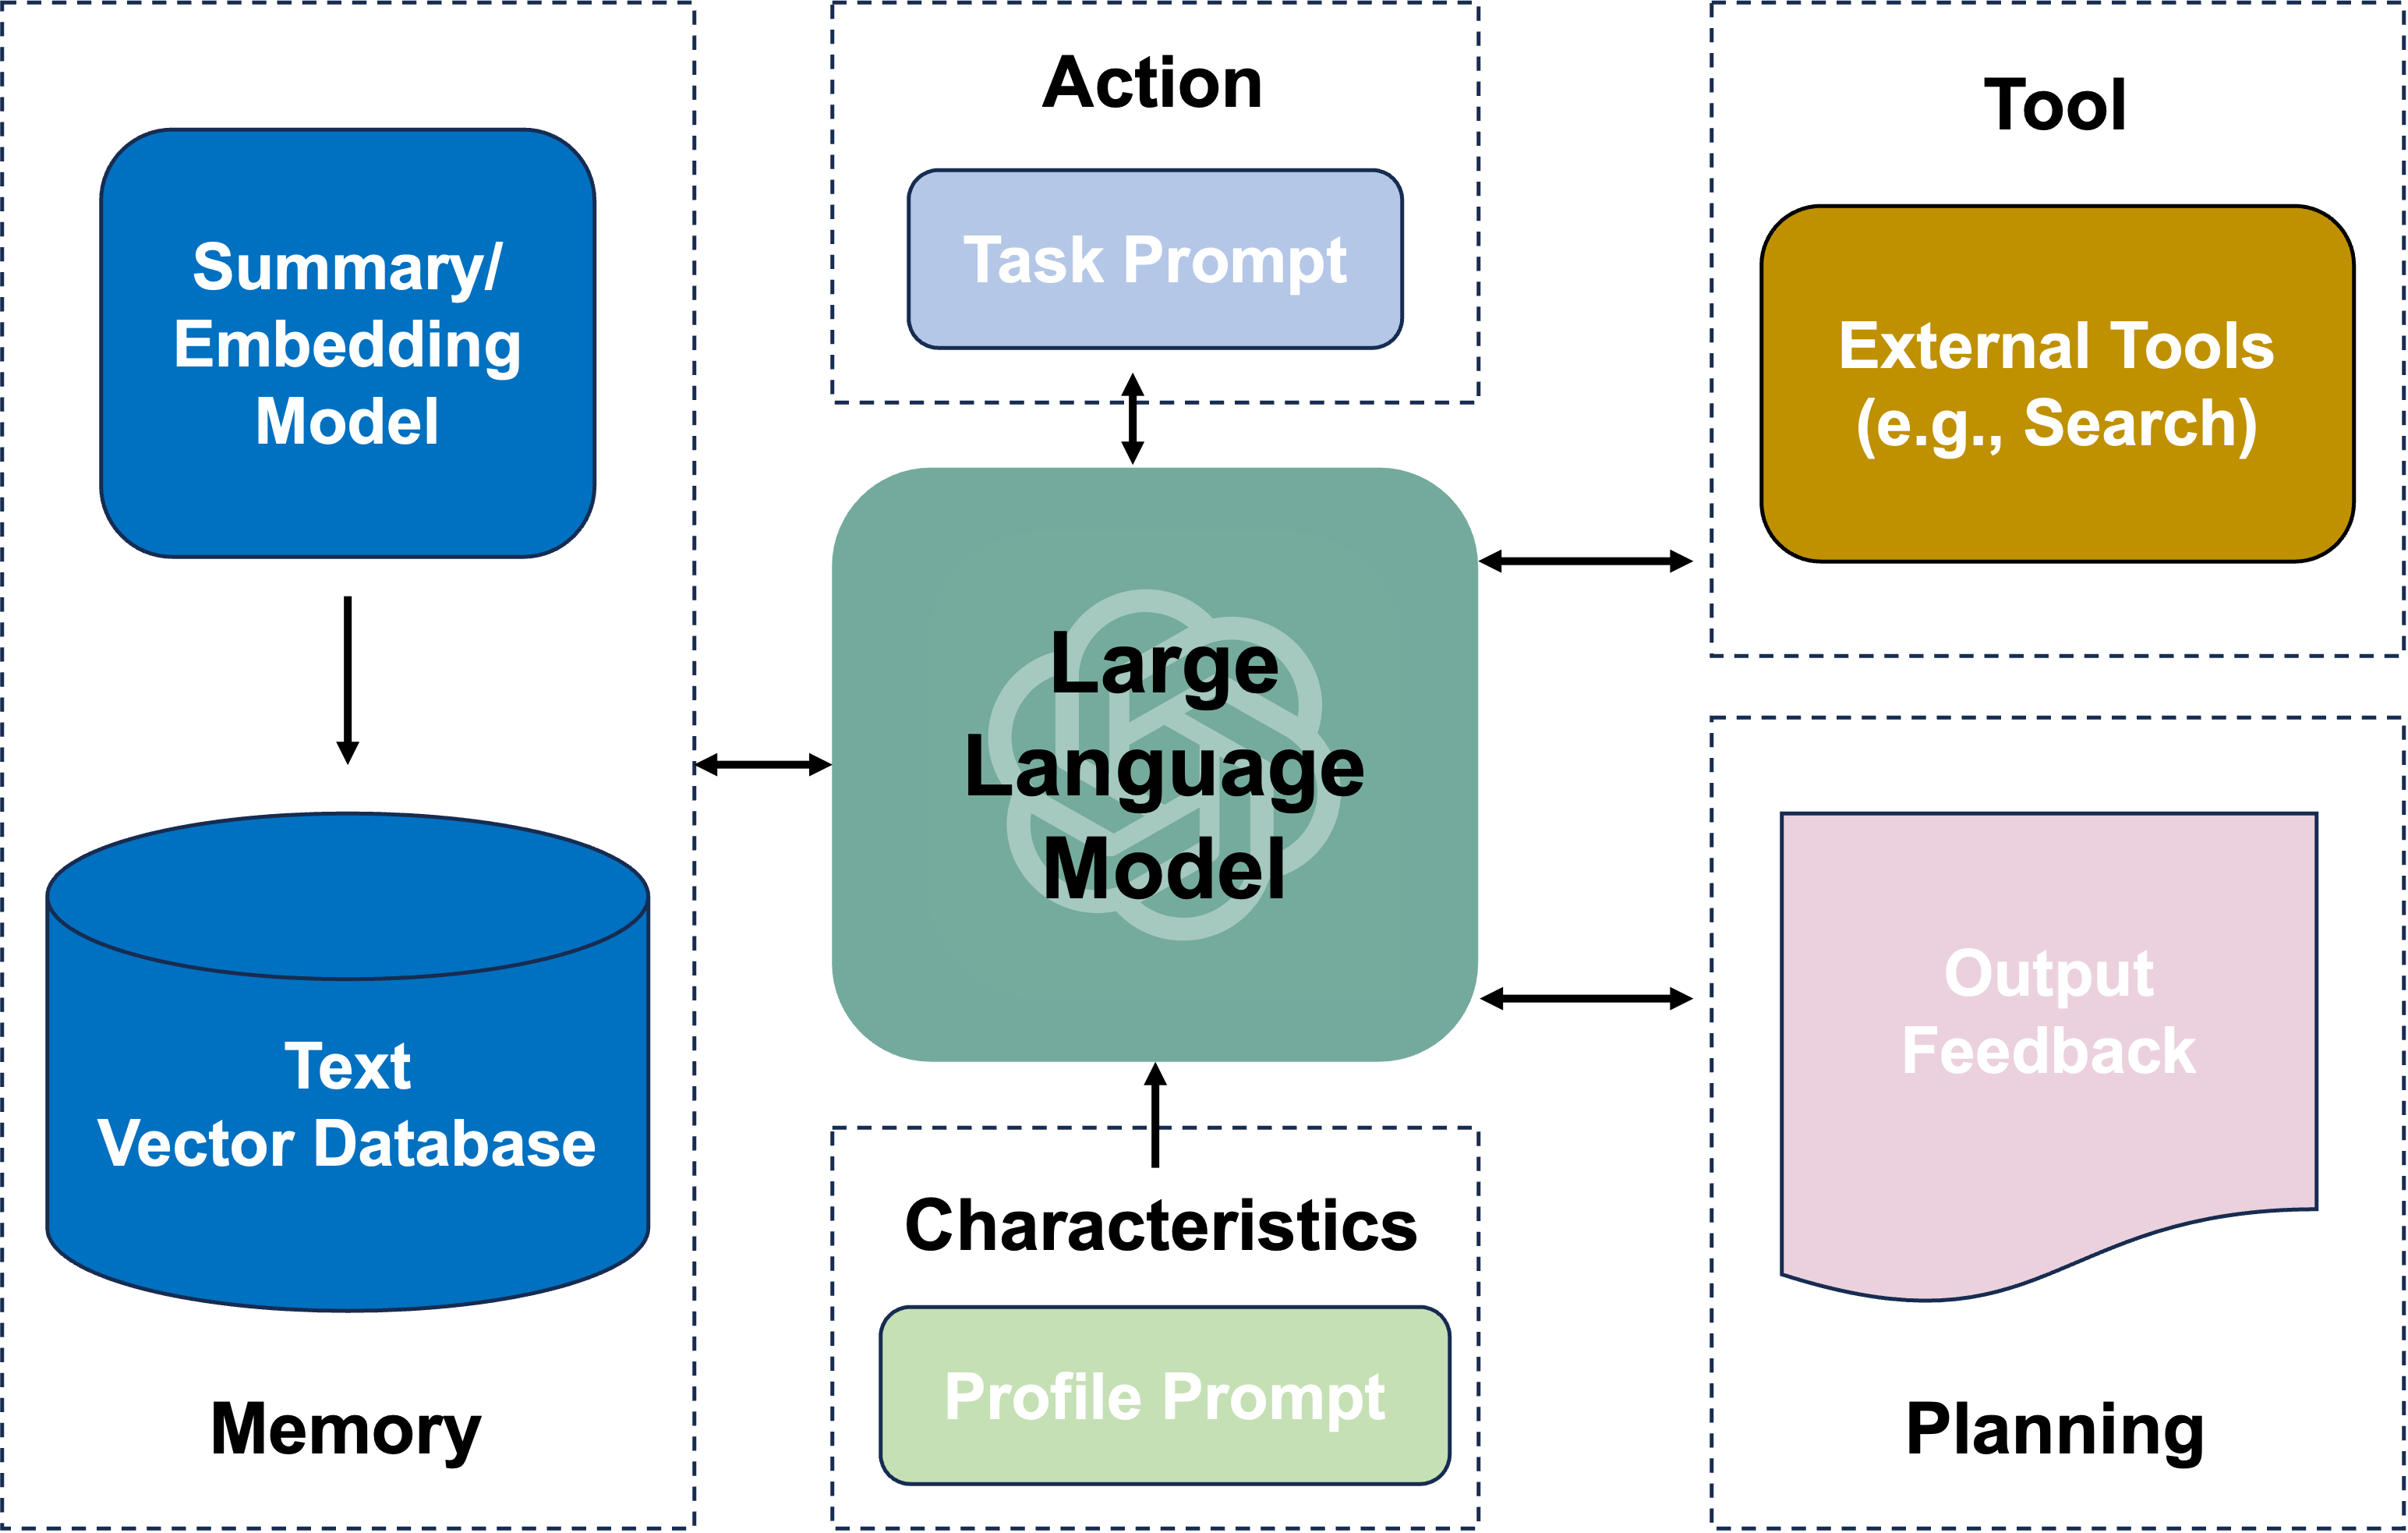
\includegraphics[width=0.6\linewidth]{Figure/llm-agent.png}
    \end{figure}
    \end{frame}

    \begin{frame}{大規模言語モデル駆動のエージェント}{\secname : 社会シミュレーション}
    \begin{itemize}
    \item 大規模言語モデルは多様な人口学属性、社会経済属性、信念と認知を持つ人間の行動と意思決定を再現することができる
    \end{itemize}
    \begin{block}{Prompt of Initialing Agents}
    Role play this person. 
    
    Ideologically, you are \boldcolor{\{ideology\}}. Regarding party support, you align with \boldcolor{\{party\}}.
    
    Please tell me about your opinions about \boldcolor{\{issue\}}.
    
    Additionally, please provide a score to assess your view of \boldcolor{\{policy\}}, ranging from 0 (entirely disagree) to 10 (entirely agree).
    \end{block}
    \end{frame}

    \begin{frame}{エージェントの拡張: Memory}{\secname : 社会シミュレーション}
    \begin{itemize}
    \item エージェントにおける「\boldcolor{Memory（記憶）}」は、エージェントが対話やインタラクションを通じて得た情報を保存し、後の応答や行動に活用する機能
    \end{itemize}
    \begin{figure}
    \centering
    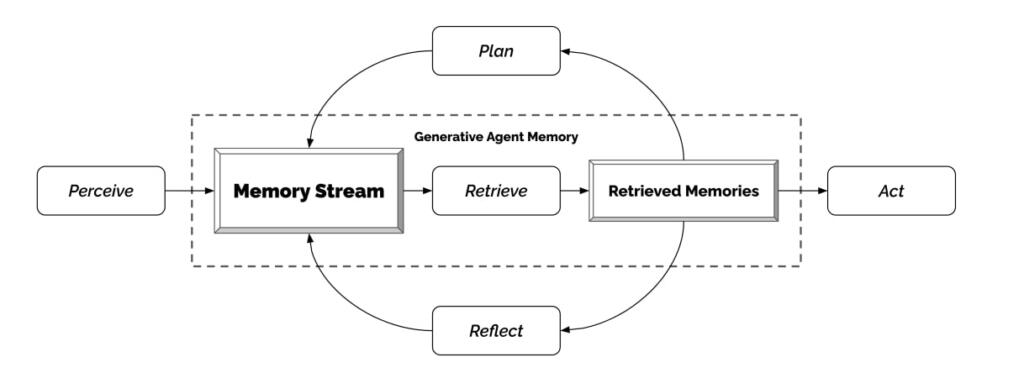
\includegraphics[width=\linewidth]{Figure/generative-ai3.png}
    \end{figure}
    \end{frame}

    \begin{frame}{エージェントの拡張: Memory}{\secname : 社会シミュレーション}
    \begin{columns}
        % Column for text
        \begin{column}{0.5\textwidth}
            \begin{itemize}
                \item エージェントは自分自身の「生活」を送り、目を覚ましや朝食を準備など日常的なルーチンをこなす
                \item 他のエージェントと交流し、記憶を保持し、計画を立てて行動する
            \end{itemize}
        \end{column}
        % Column for the image
        \begin{column}{0.5\textwidth}
            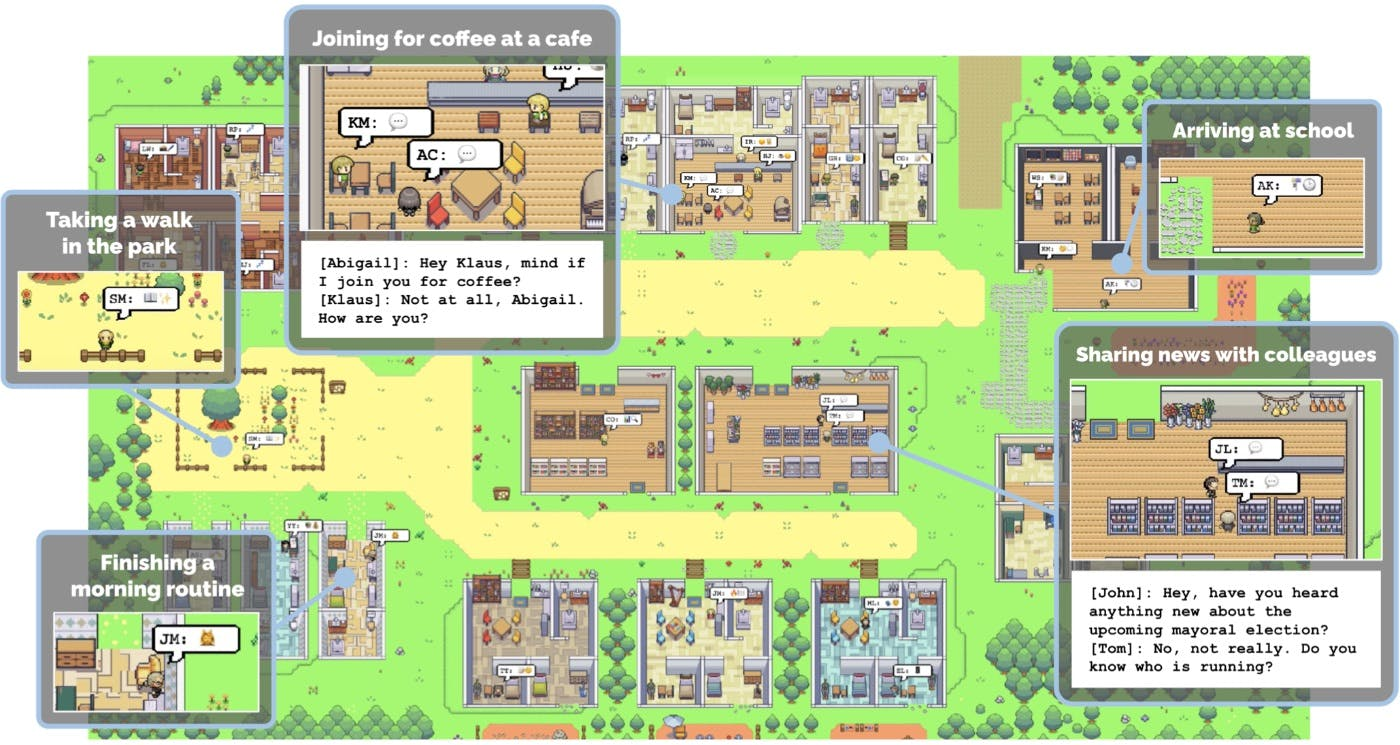
\includegraphics[width=\textwidth]{Figure/generative-ai.png} % Adjust the path to your image
        \end{column}
    \end{columns}
    \pause
    \begin{block}{}
    記憶機能により、過去の状況と交流履歴を加味しつつ自身の状況をアップデートすることができるため、長期的な相互作用過程を再現する
    \begin{itemize}
        \item Agents同士で相談しながら問題解決
        \item Agents同士の交流により成り立つ社会行動
    \end{itemize}
    \end{block}
    \rfootnote{Park, J. S., O’Brien, J. C., Cai, C. J., Morris, M. R., Liang, P., & Bernstein, M. S. (2023). Generative Agents: Interactive Simulacra of Human Behavior. ArXiv.}
    \end{frame}

    \begin{frame}{エージェントの拡張: ツール}{\secname : 社会シミュレーション}
    \begin{itemize}
    \item エージェントの「ツール」とは、エージェントが特定のタスクを遂行するために利用できる外部機能やリソースを指す
    \begin{itemize}
        \item エージェントはその本来の能力を超えて、より高度で多様な問題を解決することが可能になる
        \item リアルタイムのデータや外部リソースにアクセスし、応答の質を高める
        \item 特定分野に特化したツールを使用して、専門的な問題を解決
    \end{itemize}
    \end{itemize}
    \end{frame}

    \begin{frame}{エージェントの拡張: ツール}{\secname : 社会シミュレーション}
    \begin{figure}
    \centering
    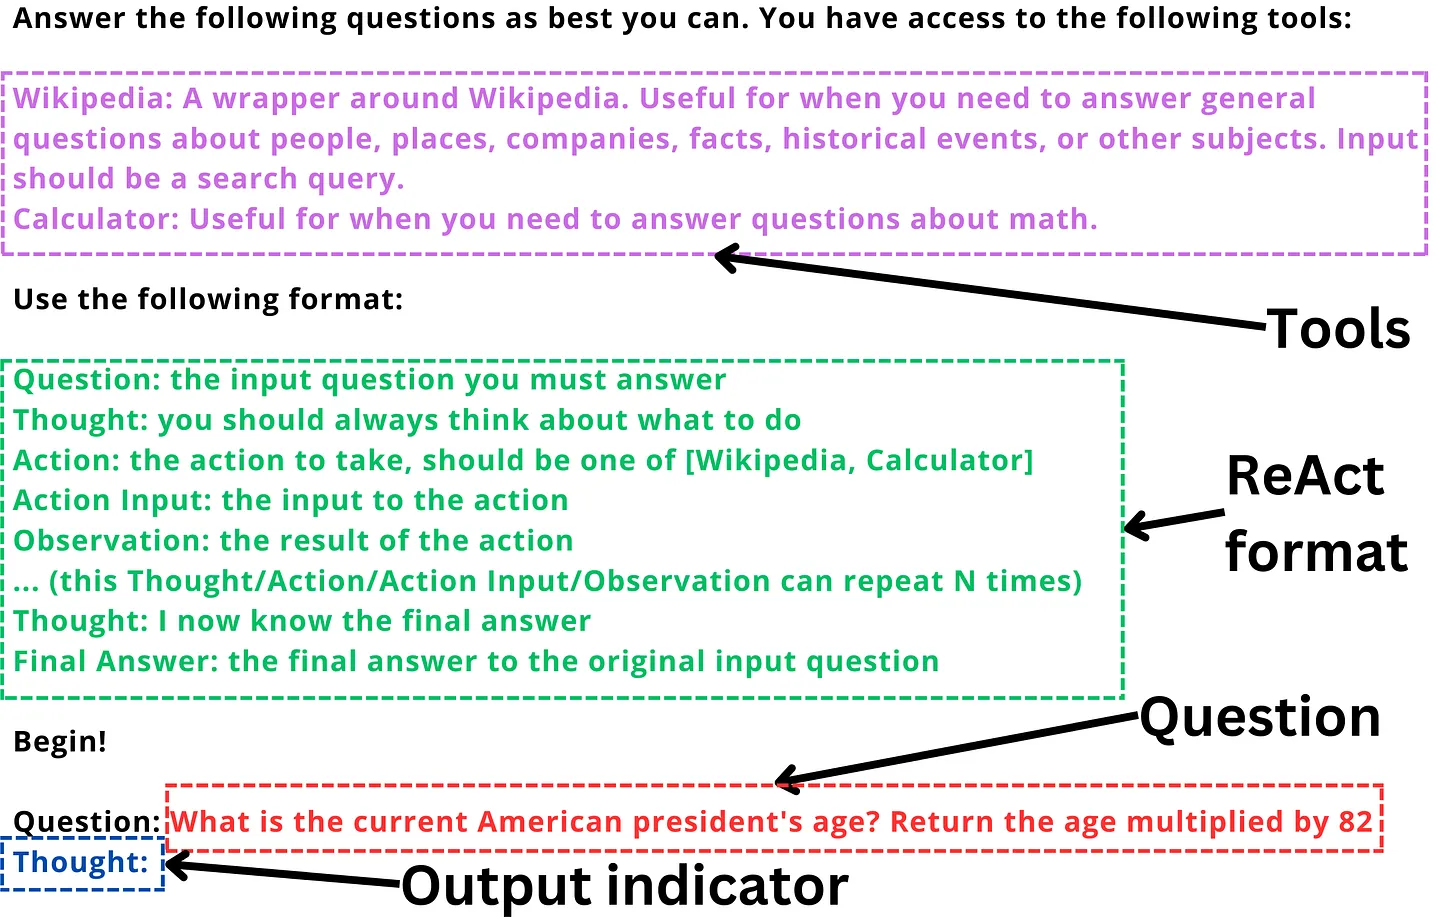
\includegraphics[width=0.75\linewidth]{Figure/agent1.png}
    \end{figure}
    \end{frame}

    \begin{frame}{エージェントの拡張: ツール}{\secname : 社会シミュレーション}
    \begin{figure}
    \centering
    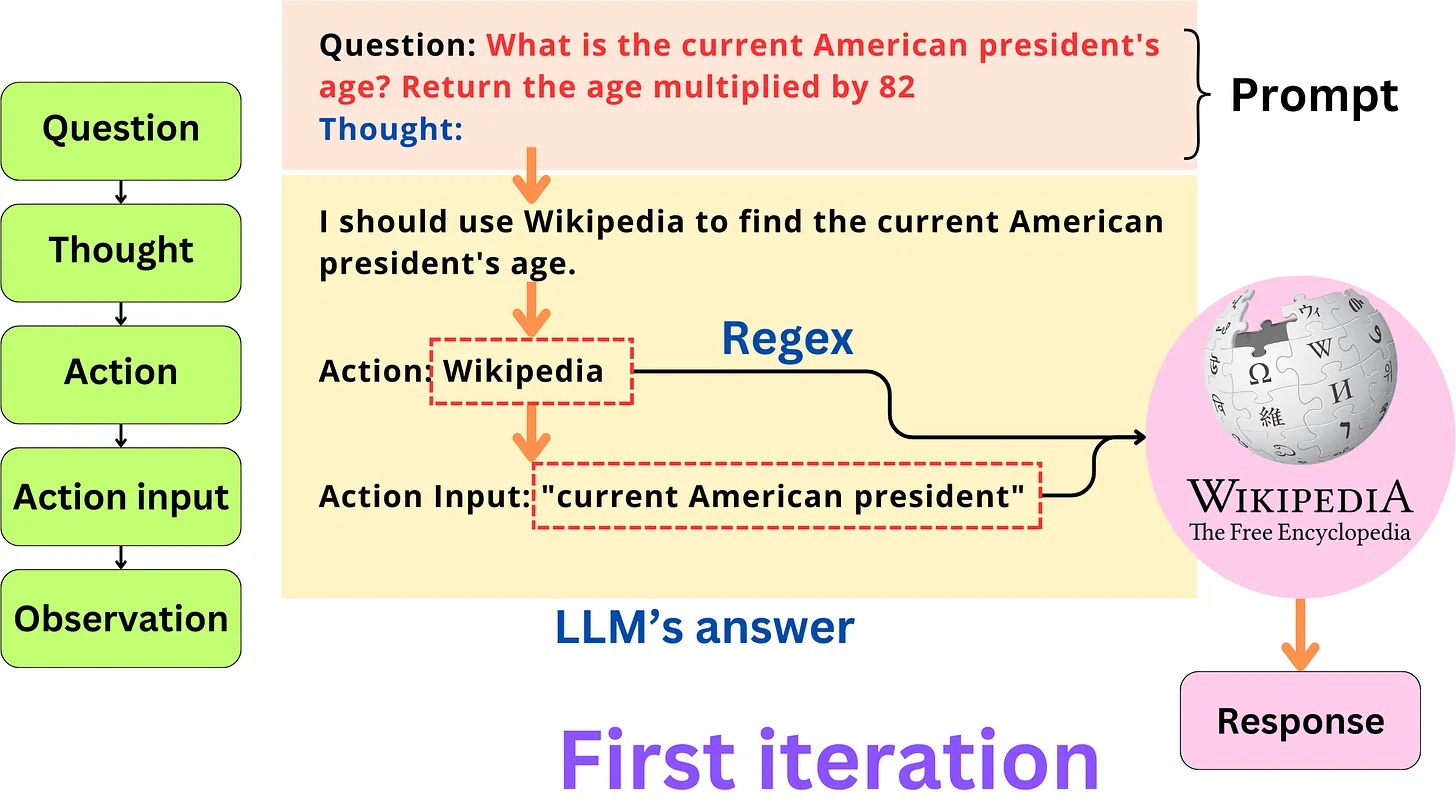
\includegraphics[width=0.75\linewidth]{Figure/agent2.png}
    \end{figure}
    \end{frame}
    
    \begin{frame}{エージェントの拡張: ツール}{\secname : 社会シミュレーション}
    \begin{figure}
    \centering
    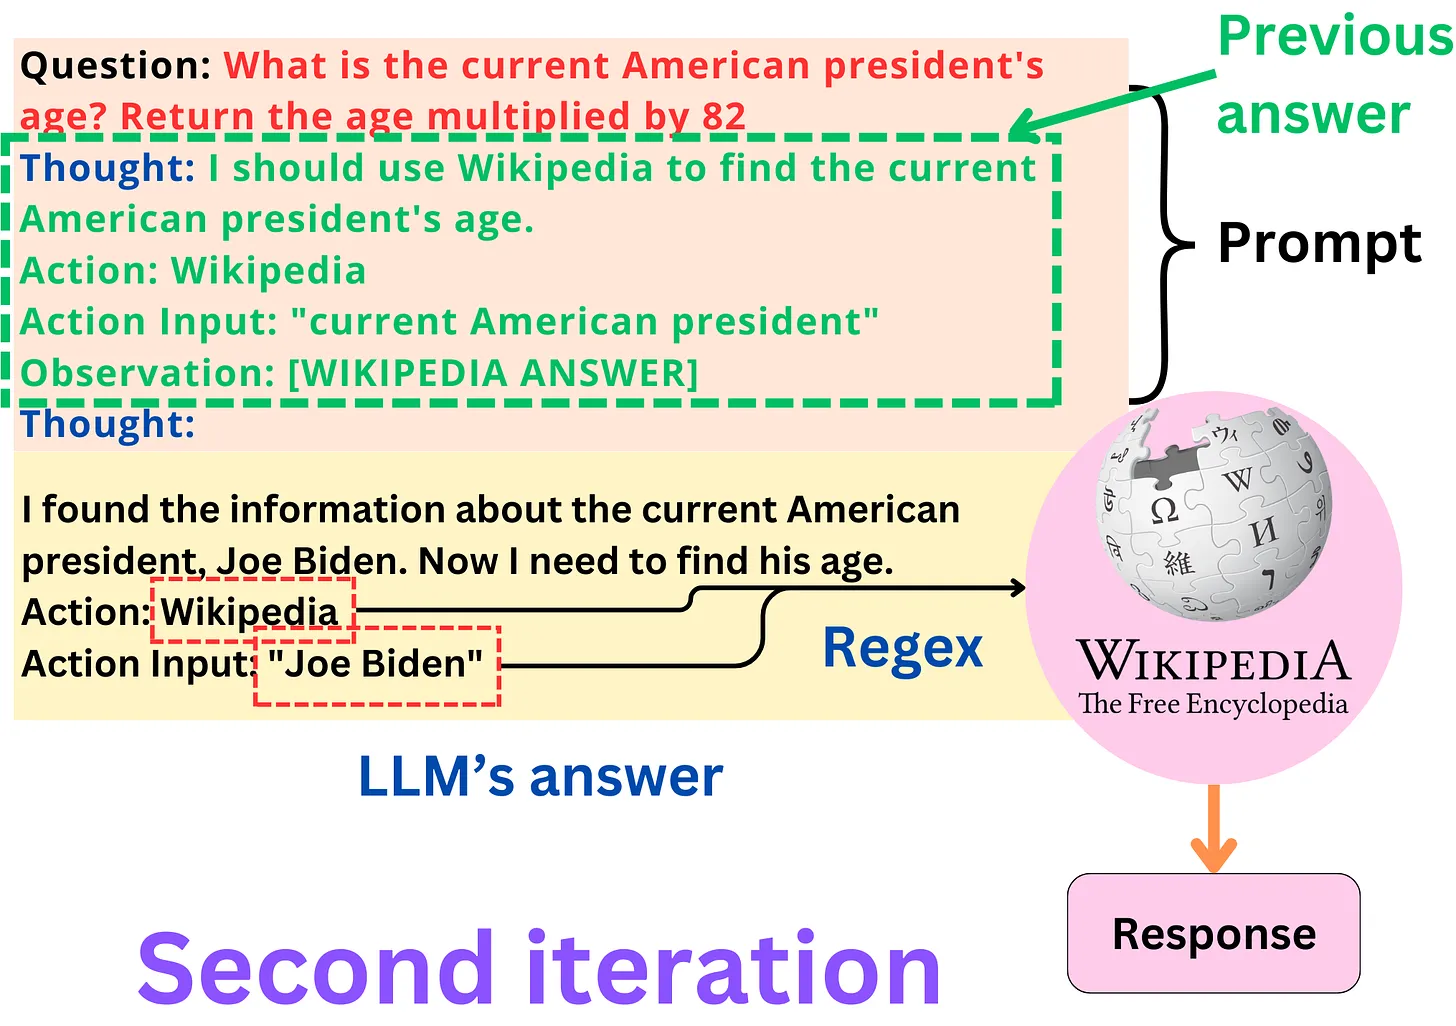
\includegraphics[width=0.72\linewidth]{Figure/agent3.png}
    \end{figure}
    \end{frame}

    \begin{frame}{エージェントの拡張: ツール}{\secname : 社会シミュレーション}
    \begin{figure}
    \centering
    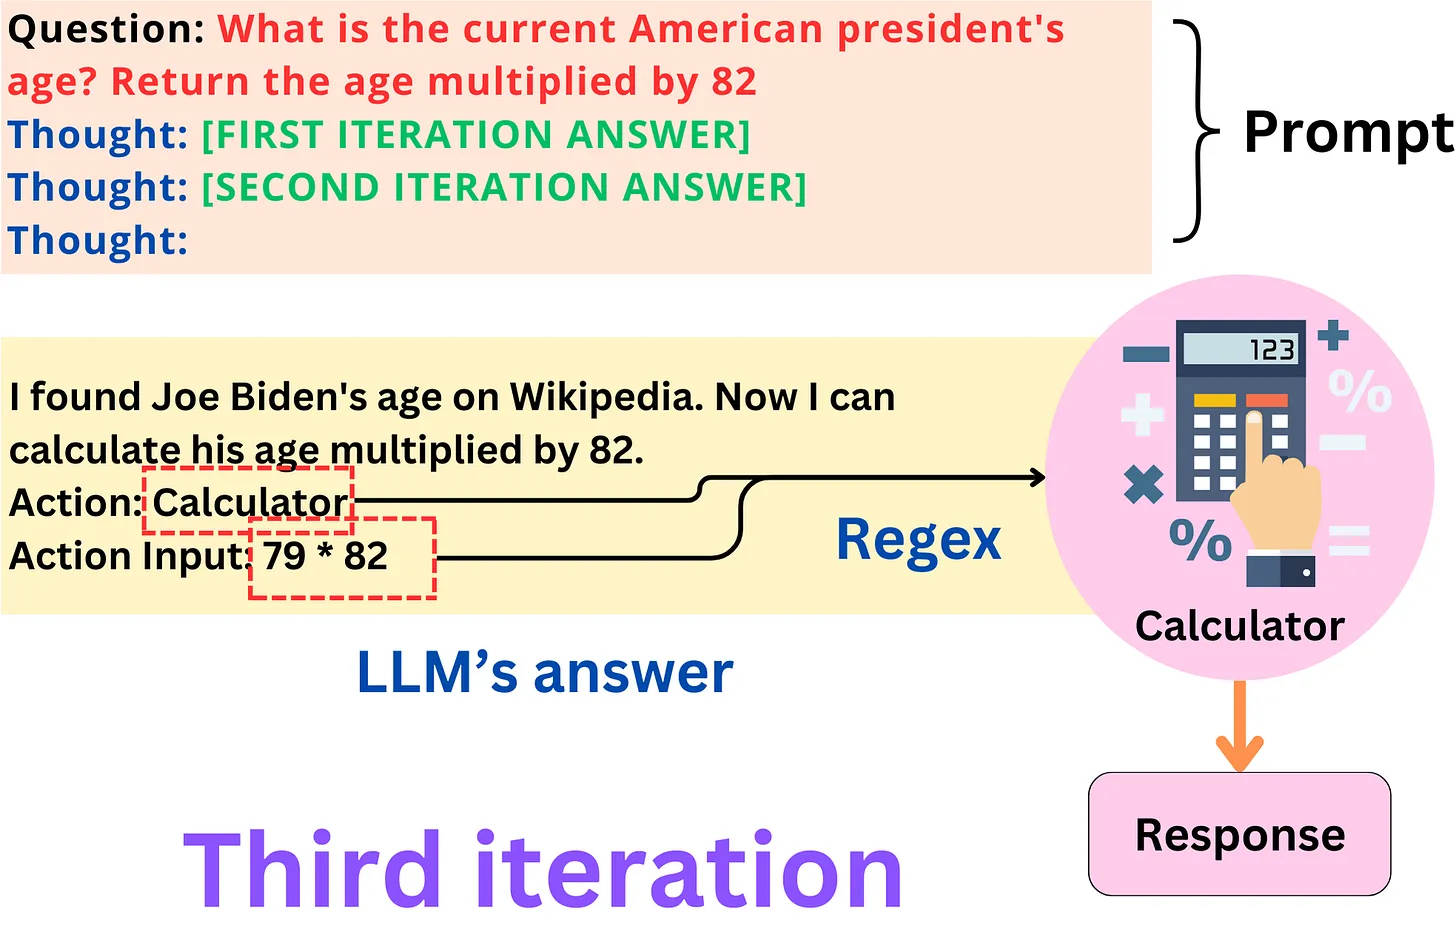
\includegraphics[width=0.75\linewidth]{Figure/agent4.png}
    \end{figure}
    \end{frame}

    \begin{frame}{エージェントの拡張: ツール}{\secname : 社会シミュレーション}
    \begin{figure}
    \centering
    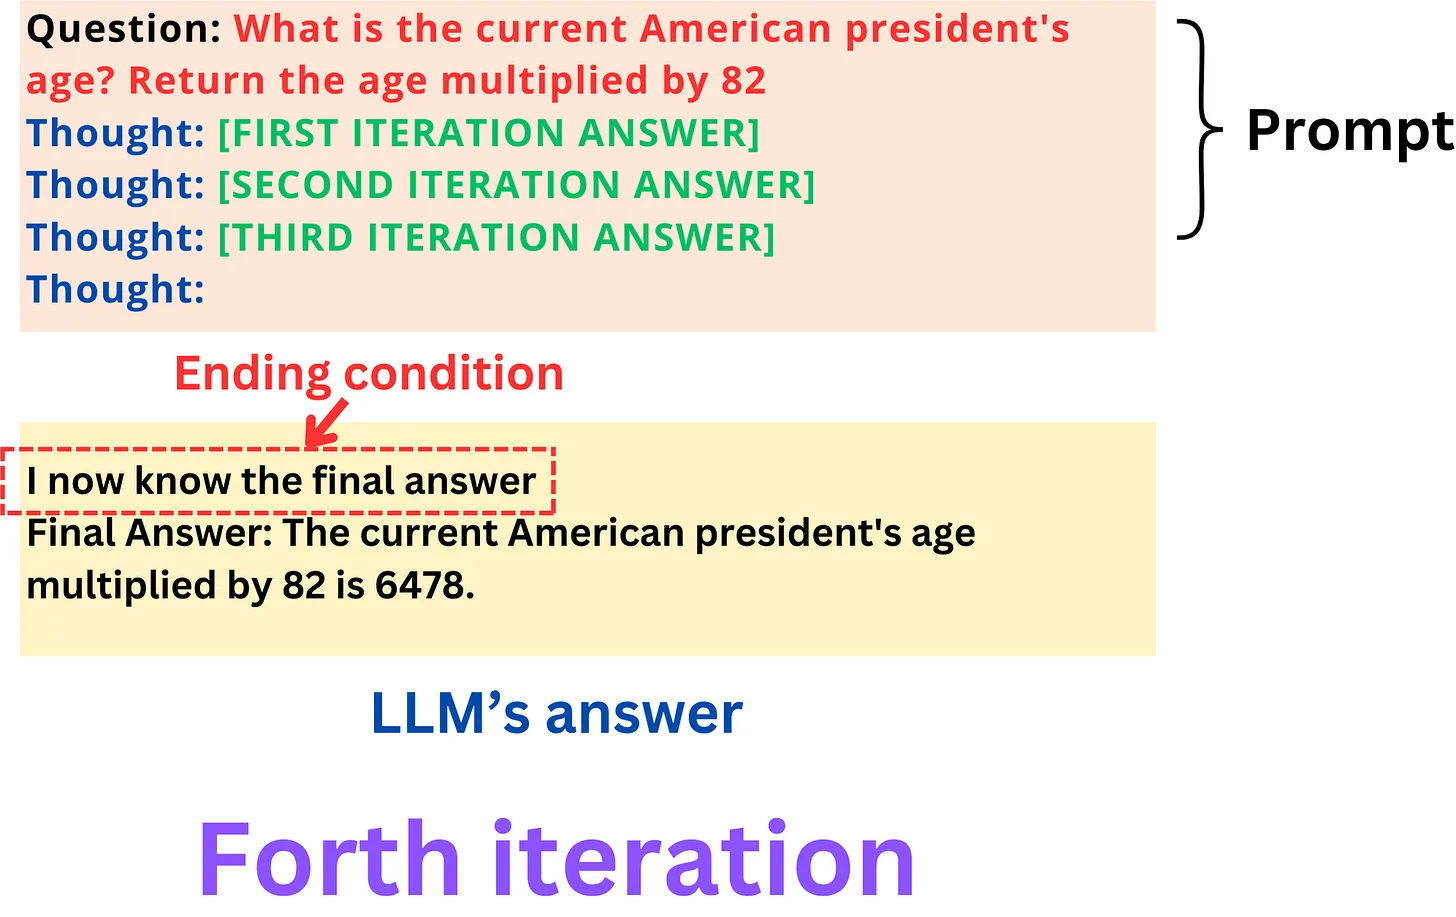
\includegraphics[width=0.75\linewidth]{Figure/agent5.png}
    \end{figure}
    \end{frame}

    \begin{frame}{エージェントの拡張: ツール}{\secname : 社会シミュレーション}
    \begin{figure}
    \centering
    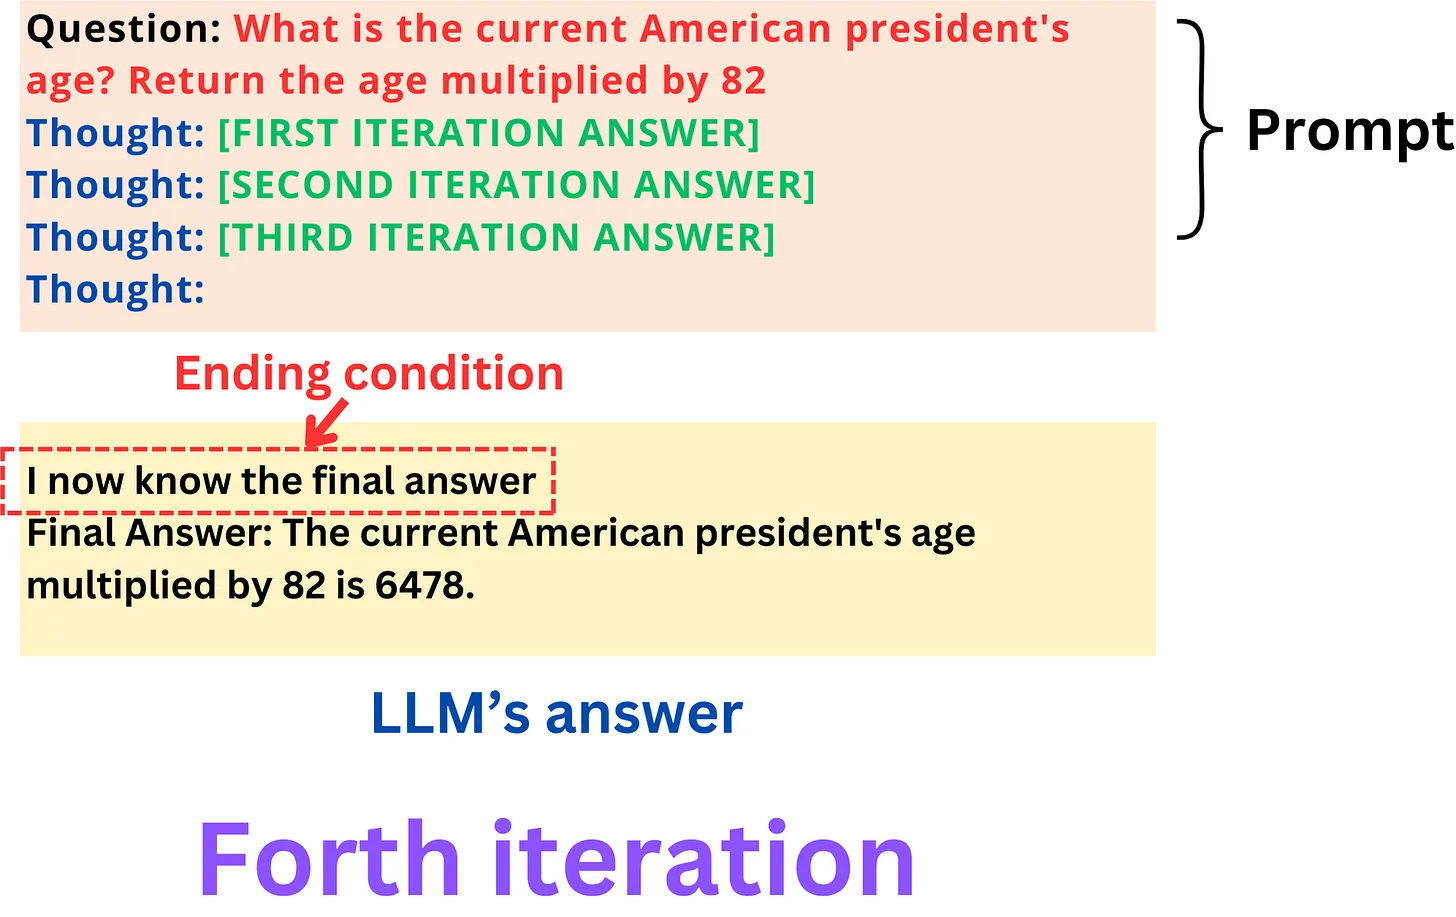
\includegraphics[width=0.75\linewidth]{Figure/agent5.png}
    \end{figure}
    \end{frame}

    \begin{frame}{マルチエージェントシステム}{\secname : 社会シミュレーション}
    \begin{figure}
    \centering
    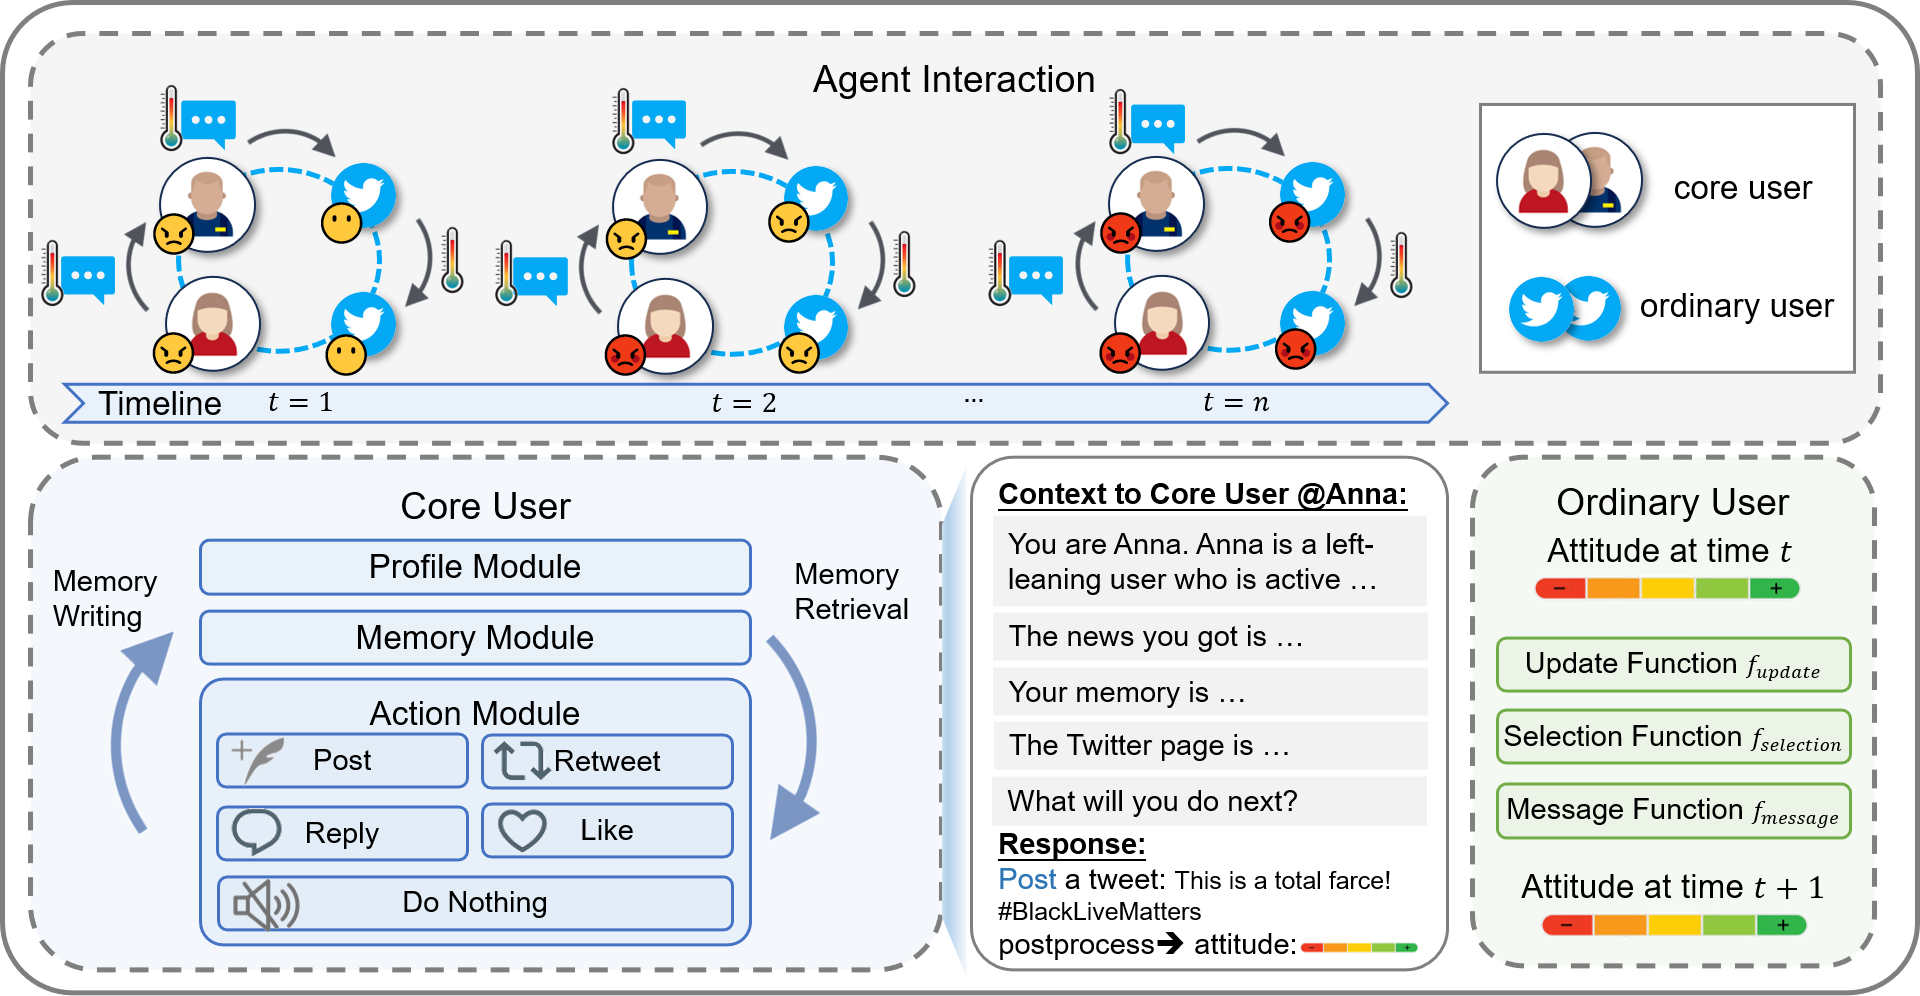
\includegraphics[width=0.75\linewidth]{Figure/llm-social-movebment.png}
    \end{figure}
    \rfootnote{Mou, X. et al. (2024). Unveiling the Truth and Facilitating Change: Towards Agent-based Large-scale Social Movement Simulation. ArXiv. \href{https://arxiv.org/abs/2402.16333}{https://arxiv.org/abs/2402.16333}.} 
    \end{frame}

    \section{まとめ}
    \begin{frame}{今後の展望}{\secname}
    \begin{itemize}
        \item \textbf{大規模言語モデルそして拡張方法とツールの発展が、社会科学研究に新たな可能性をもたらす}
        \begin{itemize}
            \item 先行研究の限界を超える
            \item 新しい研究方向の創出
        \end{itemize}
        \item \textbf{社会科学研究は大規模言語モデルの発展に貢献できる}
        \begin{itemize}
            \item 大規模言語モデル解釈可能性の向上
            \item 大規模言語モデル評価基準の確立
        \end{itemize}


    \end{itemize}
    \end{frame}
\end{document}
